\section[Intro]{Introduction}
%%%%%%%%%%%%%%%%%%%%%%%%%%%%%%%%%%%%%%%%%%%%%%%%%%%%%%%%%%%%%%%%%%%%%%%%%%%%%%%%%%
\begin{frame}[fragile]\frametitle{}
\begin{center}
{\Large Introduction}
\end{center}
\end{frame}


%%%%%%%%%%%%%%%%%%%%%%%%%%%%%%%%%%%%%%%%%%%%%%%%%%%%%%%%%%%%%%%%%%%%%%%%%%%%%%%%%%
\begin{frame}\frametitle{A graph is}
{\emph \ldots a set of discrete objects, each of which has some set of relationships with the other objects}

Abstraction:

\begin{center}
\includegraphics[width=\linewidth,keepaspectratio]{neo4j4}
\end{center}	  

{\tiny (Ref: Introduction to Neo4j - a hands-on crash course - neo4j)}
\end{frame}


%%%%%%%%%%%%%%%%%%%%%%%%%%%%%%%%%%%%%%%%%%%%%%%%%%%%%%%%%%%%%%%%%%%%%%%%%%%%%%%%%%
\begin{frame}\frametitle{Graph Theory}

\begin{itemize}
\item 
\end{itemize}



{\tiny (Ref: A Little Graph Theory for the Busy Developer - Jim Webber GraphConnect London 2013)}
\end{frame}

%%%%%%%%%%%%%%%%%%%%%%%%%%%%%%%%%%%%%%%%%%%%%%%%%%%%%%%%%%%
\begin{frame}[fragile]\frametitle{ Graph-structured Data Are Ubiquitous }

\begin{center}
\includegraphics[width=\linewidth,keepaspectratio]{gnn1}
\end{center}	  

\end{frame}

%%%%%%%%%%%%%%%%%%%%%%%%%%%%%%%%%%%%%%%%%%%%%%%%%%%%%%%%%%%
\begin{frame}[fragile]\frametitle{}

\begin{center}
\includegraphics[width=\linewidth,keepaspectratio]{gnn2}
\end{center}	  

\end{frame}

%%%%%%%%%%%%%%%%%%%%%%%%%%%%%%%%%%%%%%%%%%%%%%%%%%%%%%%%%%%
\begin{frame}[fragile]\frametitle{}

\begin{center}
\includegraphics[width=\linewidth,keepaspectratio]{gnn3}
\end{center}	  

\end{frame}

%%%%%%%%%%%%%%%%%%%%%%%%%%%%%%%%%%%%%%%%%%%%%%%%%%%%%%%%%%%
\begin{frame}[fragile]\frametitle{Graphs: A Universal Language }

\begin{center}
\includegraphics[width=\linewidth,keepaspectratio]{gnn4}
\end{center}	  

\end{frame}


%%%%%%%%%%%%%%%%%%%%%%%%%%%%%%%%%%%%%%%%%%%%%%%%%%%%%%%%%%%
\begin{frame}[fragile]\frametitle{Data as Graphs - Explicit }

\begin{center}
\includegraphics[width=\linewidth,keepaspectratio]{gnn5}
\end{center}	  

\end{frame}

%%%%%%%%%%%%%%%%%%%%%%%%%%%%%%%%%%%%%%%%%%%%%%%%%%%%%%%%%%%
\begin{frame}[fragile]\frametitle{Data as Graphs - Implicit }

\begin{center}
\includegraphics[width=\linewidth,keepaspectratio]{gnn6}
\end{center}	  

\end{frame}



%%%%%%%%%%%%%%%%%%%%%%%%%%%%%%%%%%%%%%%%%%%%%%%%%%%%%%%%%%%
\begin{frame}[fragile]\frametitle{}

\begin{center}
\includegraphics[width=\linewidth,keepaspectratio]{gnn8}
\end{center}	  

\end{frame}


%%%%%%%%%%%%%%%%%%%%%%%%%%%%%%%%%%%%%%%%%%%%%%%%%%%%%%%%%%%%%%%%%%%%%%%%%%%%%%%%%%
\begin{frame}\frametitle{Graph Components}

\begin{itemize}
\item Node (Vertex): A must data element for constructing a graph
\item Relationship (Edge) : Link between two nodes, can have direction and type.
\item Label: Node category/type such as PERSON, ORG, etc. One node can have many types.
\item Properties: Attributes or fields in Nodes or Edges, eg. A node can have Label PERSON and Property such as ``name: Jane''
\end{itemize}



{\tiny (Ref: Introduction to Neo4j - a hands-on crash course - neo4j)}
\end{frame}


%%%%%%%%%%%%%%%%%%%%%%%%%%%%%%%%%%%%%%%%%%%%%%%%%%%%%%%%%%%%%%%%%%%%%%%%%%%%%%%%%%
\begin{frame}\frametitle{Nodes}


\begin{center}
\includegraphics[width=\linewidth,keepaspectratio]{neo4j33}
\end{center}	

{\tiny (Ref: CIS 6930 - Advanced Databases - Neo4j )}
\end{frame}


%%%%%%%%%%%%%%%%%%%%%%%%%%%%%%%%%%%%%%%%%%%%%%%%%%%%%%%%%%%%%%%%%%%%%%%%%%%%%%%%%%
\begin{frame}\frametitle{Relationships}


\begin{center}
\includegraphics[width=\linewidth,keepaspectratio]{neo4j34}
\end{center}	

{\tiny (Ref: CIS 6930 - Advanced Databases - Neo4j )}
\end{frame}

%%%%%%%%%%%%%%%%%%%%%%%%%%%%%%%%%%%%%%%%%%%%%%%%%%%%%%%%%%%%%%%%%%%%%%%%%%%%%%%%%%
\begin{frame}\frametitle{Properties}


\begin{center}
\includegraphics[width=\linewidth,keepaspectratio]{neo4j35}
\end{center}	

{\tiny (Ref: CIS 6930 - Advanced Databases - Neo4j )}
\end{frame}


%%%%%%%%%%%%%%%%%%%%%%%%%%%%%%%%%%%%%%%%%%%%%%%%%%%%%%%%%%%%%%%%%%%%%%%%%%%%%%%%%%
\begin{frame}\frametitle{Labels}


\begin{center}
\includegraphics[width=\linewidth,keepaspectratio]{neo4j36}
\end{center}	

{\tiny (Ref: CIS 6930 - Advanced Databases - Neo4j )}
\end{frame}


%%%%%%%%%%%%%%%%%%%%%%%%%%%%%%%%%%%%%%%%%%%%%%%%%%%%%%%%%%%
\begin{frame}[fragile]\frametitle{Graphs and features}

\begin{center}
\includegraphics[width=\linewidth,keepaspectratio]{gnn9}
\end{center}	  

\end{frame}

%%%%%%%%%%%%%%%%%%%%%%%%%%%%%%%%%%%%%%%%%%%%%%%%%%%%%%%%%%%
\begin{frame}[fragile]\frametitle{Matrix Representations of Graphs}

\begin{center}
\includegraphics[width=\linewidth,keepaspectratio]{gnn10}
\end{center}	  

\end{frame}

%%%%%%%%%%%%%%%%%%%%%%%%%%%%%%%%%%%%%%%%%%%%%%%%%%%%%%%%%%%
\begin{frame}[fragile]\frametitle{Why Graphs? Why Now?}

\begin{itemize}
\item Universal language for describing complex data: Networks/graphs from science, nature, and technology are more similar than one would expect
\item Shared vocabulary between fields: Computer Science, Social science, Physics, Biology, Economics 
\item Data availability (+ computational challenges): Social/Internet, text, logic, program, bio, health, and medical
\item Impact: Social networking, Social media, Drug design, Event detection, Natural language processing, Computer vision, and Logic reasoning
\end{itemize}

\end{frame}

%%%%%%%%%%%%%%%%%%%%%%%%%%%%%%%%%%%%%%%%%%%%%%%%%%%%%%%%%%%%%%%%%%%%%%%%%%%%%%%%%%
\begin{frame}\frametitle{Identifying good Graph scenarios - 1/4}

Does the problem involve understanding relationships between entities?

Behavioral analysis:

\begin{center}
\includegraphics[width=\linewidth,keepaspectratio]{neo4j5}
\end{center}	  

{\tiny (Ref: Introduction to Neo4j - a hands-on crash course - neo4j)}
\end{frame}

%%%%%%%%%%%%%%%%%%%%%%%%%%%%%%%%%%%%%%%%%%%%%%%%%%%%%%%%%%%%%%%%%%%%%%%%%%%%%%%%%%
\begin{frame}\frametitle{Identifying good Graph scenarios - 2/4}

Does the problem involve a lot of self-referencing to the same type of entity?

Org chart of employees:

\begin{center}
\includegraphics[width=\linewidth,keepaspectratio]{neo4j6}
\end{center}	  

{\tiny (Ref: Introduction to Neo4j - a hands-on crash course - neo4j)}
\end{frame}

%%%%%%%%%%%%%%%%%%%%%%%%%%%%%%%%%%%%%%%%%%%%%%%%%%%%%%%%%%%%%%%%%%%%%%%%%%%%%%%%%%
\begin{frame}\frametitle{Identifying good Graph scenarios - 3/4}

Does the problem explore relationships of varying and unknown depth?

Changes in manufacturing process:

\begin{center}
\includegraphics[width=\linewidth,keepaspectratio]{neo4j7}
\end{center}	  

{\tiny (Ref: Introduction to Neo4j - a hands-on crash course - neo4j)}
\end{frame}

%%%%%%%%%%%%%%%%%%%%%%%%%%%%%%%%%%%%%%%%%%%%%%%%%%%%%%%%%%%%%%%%%%%%%%%%%%%%%%%%%%
\begin{frame}\frametitle{Identifying good Graph scenarios - 4/4}

Does the problem involve discovering lots of different routes or paths?

Optimum logistics:

\begin{center}
\includegraphics[width=\linewidth,keepaspectratio]{neo4j8}
\end{center}	  

{\tiny (Ref: Introduction to Neo4j - a hands-on crash course - neo4j)}
\end{frame}




\section[Db]{Databases}
%%%%%%%%%%%%%%%%%%%%%%%%%%%%%%%%%%%%%%%%%%%%%%%%%%%%%%%%%%%%%%%%%%%%%%%%%%%%%%%%%%
\begin{frame}[fragile]\frametitle{}
\begin{center}
{\Large Database}
\end{center}
\end{frame}

%%%%%%%%%%%%%%%%%%%%%%%%%%%%%%%%%%%%%%%%%%%%%%%%%%%%%%%%%%%%%%%%%%%%%%%%%%%%%%%%%%
\begin{frame}\frametitle{A Brief DB History}

Early 1970s

\begin{itemize}
\item Many database systems
\item Incompatible, exposing many implementation details
\end{itemize}

Then Ted Codd came along
\begin{itemize}
\item Relational model
\item Structured Query Language (SQL)
\item Implementation differences became irrelevant
\item A few major DB systems dominated the market
\end{itemize}


{\tiny (Ref: Are Relational Databases the Only Type of Databases? )}
\end{frame}


%%%%%%%%%%%%%%%%%%%%%%%%%%%%%%%%%%%%%%%%%%%%%%%%%%%%%%%%%%%%%%%%%%%%%%%%%%%%%%%%%%
\begin{frame}\frametitle{Architecture Changes Over Time }
1980’s: Single Application


\begin{center}
\includegraphics[width=0.2\linewidth,keepaspectratio]{neo4j52}
\end{center}	

{\tiny (Ref: NoSQL: Graph Databases)}

\end{frame}

%%%%%%%%%%%%%%%%%%%%%%%%%%%%%%%%%%%%%%%%%%%%%%%%%%%%%%%%%%%%%%%%%%%%%%%%%%%%%%%%%%
\begin{frame}\frametitle{Architecture Changes Over Time }
Database Anti-pattern


\begin{center}
\includegraphics[width=\linewidth,keepaspectratio]{neo4j53}
\end{center}	

{\tiny (Ref: NoSQL: Graph Databases)}

\end{frame}


%%%%%%%%%%%%%%%%%%%%%%%%%%%%%%%%%%%%%%%%%%%%%%%%%%%%%%%%%%%%%%%%%%%%%%%%%%%%%%%%%%
\begin{frame}\frametitle{Architecture Changes Over Time }
2000’s: SOA



\begin{center}
\includegraphics[width=\linewidth,keepaspectratio]{neo4j54}
\end{center}	

{\tiny (Ref: NoSQL: Graph Databases)}

\end{frame}


%%%%%%%%%%%%%%%%%%%%%%%%%%%%%%%%%%%%%%%%%%%%%%%%%%%%%%%%%%%%%%%%%%%%%%%%%%%%%%%%%%
\begin{frame}\frametitle{Web 1/2/3 and Big Data}


\begin{itemize}
\item Twitter: 350 million monthly active users and 500 million Tweets are sent per day,
\item Facebook: over 1 billion monthly users and faces 3 million message per 20 minute
\item Instagram: 200 Million Monthly Active Users and 1.6 Billion Likes and 60 Million Photos shared every day

\end{itemize}


{\tiny (Ref: Are Relational Databases the Only Type of Databases? )}
\end{frame}


%%%%%%%%%%%%%%%%%%%%%%%%%%%%%%%%%%%%%%%%%%%%%%%%%%%%%%%%%%%%%%%%%%%%%%%%%%%%%%%%%%
\begin{frame}\frametitle{Background}

Data is more connected:

\begin{itemize}
\item Text (content)
\item  HyperText (added pointers)
\item  RSS (joined those pointers)
\item Blogs (added pingbacks)
\item Tagging (grouped related data)
\item RDF (described connected data)
\item GGG (content + pointers + relationships + descriptions)
\end{itemize}

 

{\tiny (Ref: CIntroduction to Graph Databases - Max De Marzi )}
\end{frame}

%%%%%%%%%%%%%%%%%%%%%%%%%%%%%%%%%%%%%%%%%%%%%%%%%%%%%%%%%%%%%%%%%%%%%%%%%%%%%%%%%%
\begin{frame}\frametitle{Structured Unstructured}


\begin{center}
\includegraphics[width=0.9\linewidth,keepaspectratio]{neo4j49}
\end{center}	

{\tiny (Ref: https://www.datamation.com/big-data/structured-vs-unstructured-data.html)}
\end{frame}



%%%%%%%%%%%%%%%%%%%%%%%%%%%%%%%%%%%%%%%%%%%%%%%%%%%%%%%%%%%%%%%%%%%%%%%%%%%%%%%%%%
\begin{frame}\frametitle{Database Systems Landscape }


\begin{center}
\includegraphics[width=\linewidth,keepaspectratio]{neo4j50}
\end{center}	

{\tiny (Ref: Are Relational Databases the Only Type of Databases? )}

\end{frame}



%%%%%%%%%%%%%%%%%%%%%%%%%%%%%%%%%%%%%%%%%%%%%%%%%%%%%%%%%%%%%%%%%%%%%%%%%%%%%%%%%%
\begin{frame}\frametitle{Introduction}

\begin{itemize}
\item A Database is a place to store application data, to process and query, etc
\item Relational databases (SQL) store data in tables. Strict schema.
\item Document Db: key-value databases (no-SQL) store data in dictionaries/json. Flexi schema.
\item A Graph Database is where data is stored in graph data structure ie nodes and edges.
\end{itemize}

\begin{center}
\includegraphics[width=0.8\linewidth,keepaspectratio]{neo4j29}
\end{center}	

{\tiny (Ref: Neo4j (Graph Database) Crash Course - Laith Academy)}
\end{frame}


%%%%%%%%%%%%%%%%%%%%%%%%%%%%%%%%%%%%%%%%%%%%%%%%%%%%%%%%%%%%%%%%%%%%%%%%%%%%%%%%%%
\begin{frame}\frametitle{Graph Database }


\begin{itemize}
\item Create, Read, Update and Delete (CRUD) operations working on a graph data model. 
\item Unlike the other databases, relationships take first priority in graph databases so the foreign keys or out-of-band processing is no more necessary to link a data to another.
\item By assembling the simple abstractions of nodes and relationships into connected structures, graph databases enable us to build sophisticated models that map closely to out problem domain.
\end{itemize}


\begin{center}
\includegraphics[width=0.8\linewidth,keepaspectratio]{neo4j75}
\end{center}	

{\tiny (Ref: Learning Neo4j - Wabri Github)}
\end{frame}


%%%%%%%%%%%%%%%%%%%%%%%%%%%%%%%%%%%%%%%%%%%%%%%%%%%%%%%%%%%%%%%%%%%%%%%%%%%%%%%%%%
\begin{frame}\frametitle{Comparison }
Relational Database

\begin{center}
\includegraphics[width=0.6\linewidth,keepaspectratio]{neo4j76}
\end{center}	

And here is the corresponding graph model:


\begin{center}
\includegraphics[width=0.8\linewidth,keepaspectratio]{neo4j77}
\end{center}	

{\tiny (Ref: Learning Neo4j - Wabri Github)}
\end{frame}

%%%%%%%%%%%%%%%%%%%%%%%%%%%%%%%%%%%%%%%%%%%%%%%%%%%%%%%%%%%%%%%%%%%%%%%%%%%%%%%%%%
\begin{frame}\frametitle{Advantage }

The graph model can be more versatile and can be upgrade without efforts, for example we want to add the confederation and country:

\begin{center}
\includegraphics[width=0.8\linewidth,keepaspectratio]{neo4j78}
\end{center}	

{\tiny (Ref: Learning Neo4j - Wabri Github)}
\end{frame}


%%%%%%%%%%%%%%%%%%%%%%%%%%%%%%%%%%%%%%%%%%%%%%%%%%%%%%%%%%%%%%%%%%%%%%%%%%%%%%%%%%
\begin{frame}\frametitle{Database Systems Landscape }


\begin{center}
\includegraphics[width=0.9\linewidth,keepaspectratio]{neo4j51}
\end{center}	

{\tiny (Ref: Are Relational Databases the Only Type of Databases? )}

\end{frame}


%%%%%%%%%%%%%%%%%%%%%%%%%%%%%%%%%%%%%%%%%%%%%%%%%%%%%%%%%%%%%%%%%%%%%%%%%%%%%%%%%%
\begin{frame}\frametitle{What is a Graph Database?}

\begin{itemize}
\item A database with an explicit graph structure
\item Each node knows its adjacent nodes 
\item As the number of nodes increases, the cost of a local step (or hop) remains the same
\item Plus an Index for lookups
\end{itemize}

{\tiny (Ref: CIntroduction to Graph Databases - Max De Marzi )}
\end{frame}


%%%%%%%%%%%%%%%%%%%%%%%%%%%%%%%%%%%%%%%%%%%%%%%%%%%%%%%%%%%%%%%%%%%%%%%%%%%%%%%%%%
\begin{frame}\frametitle{Example}


\begin{center}
\includegraphics[width=\linewidth,keepaspectratio]{neo4j30}
\end{center}	

{\tiny (Ref: CIS 6930 - Advanced Databases - Neo4j )}
\end{frame}

%%%%%%%%%%%%%%%%%%%%%%%%%%%%%%%%%%%%%%%%%%%%%%%%%%%%%%%%%%%
\begin{frame}[fragile]\frametitle{Relational Database}
SQL

\begin{center}
\includegraphics[width=\linewidth,keepaspectratio]{neo4j17}
\end{center}	    

{\tiny (Ref: Introduction to Neo4j and Graph Databases
 - M David Allen)}

\end{frame}

%%%%%%%%%%%%%%%%%%%%%%%%%%%%%%%%%%%%%%%%%%%%%%%%%%%%%%%%%%%
\begin{frame}[fragile]\frametitle{Graph Database}
Cypher

\begin{center}
\includegraphics[width=\linewidth,keepaspectratio]{neo4j18}
\end{center}	    

{\tiny (Ref: Introduction to Neo4j and Graph Databases
 - M David Allen)}

\end{frame}

%%%%%%%%%%%%%%%%%%%%%%%%%%%%%%%%%%%%%%%%%%%%%%%%%%%%%%%%%%%%%%%%%%%%%%%%%%%%%%%%%%
\begin{frame}\frametitle{RDBMS}

\begin{itemize}
\item Cannot model or store data and relationships well, ie, without complexity
\item Performance degrades with umber and levels of relationships and database size
\item Query complexity grows with the need for JOINs
\item Adding new types of data and relationships requires schema redesign
\item More difficult if that needs to be done real time.
\end{itemize}

{\tiny (Ref: Neo4j (Graph Database) Crash Course - Laith Academy)}
\end{frame}

%%%%%%%%%%%%%%%%%%%%%%%%%%%%%%%%%%%%%%%%%%%%%%%%%%%%%%%%%%%%%%%%%%%%%%%%%%%%%%%%%%
\begin{frame}\frametitle{Comparing RDBMS to Graph database}

\begin{center}
\includegraphics[width=\linewidth,keepaspectratio]{neo4j39}
\end{center}	  


{\tiny (Ref: CIS 6930 - Advanced Databases - Neo4j )}
\end{frame}

%%%%%%%%%%%%%%%%%%%%%%%%%%%%%%%%%%%%%%%%%%%%%%%%%%%%%%%%%%%%%%%%%%%%%%%%%%%%%%%%%%
\begin{frame}\frametitle{Comparing RDBMS to Graph database}

\begin{center}
\includegraphics[width=\linewidth,keepaspectratio]{neo4j43}
\end{center}	  


{\tiny (Ref: CIntroduction to Graph Databases - Max De Marzi )}
\end{frame}

%%%%%%%%%%%%%%%%%%%%%%%%%%%%%%%%%%%%%%%%%%%%%%%%%%%%%%%%%%%%%%%%%%%%%%%%%%%%%%%%%%
\begin{frame}\frametitle{Comparing Key Value Stores to Graph database}

\begin{center}
\includegraphics[width=\linewidth,keepaspectratio]{neo4j44}
\end{center}	  


{\tiny (Ref: CIntroduction to Graph Databases - Max De Marzi )}
\end{frame}

%%%%%%%%%%%%%%%%%%%%%%%%%%%%%%%%%%%%%%%%%%%%%%%%%%%%%%%%%%%%%%%%%%%%%%%%%%%%%%%%%%
\begin{frame}\frametitle{Comparing Key Value Stores to Graph database}

\begin{center}
\includegraphics[width=\linewidth,keepaspectratio]{neo4j45}
\end{center}	  


{\tiny (Ref: CIntroduction to Graph Databases - Max De Marzi )}
\end{frame}




% %%%%%%%%%%%%%%%%%%%%%%%%%%%%%%%%%%%%%%%%%%%%%%%%%%%%%%%%%%%%%%%%%%%%%%%%%%%%%%%%%%
% \begin{frame}\frametitle{Comparing the Joins and Cypher Query}

% We want to see who bought Chocolade. Let’s join the four tables together in Relational Model


% \begin{lstlisting}
% SELECT DISTINCT c.CompanyName
% FROM customers AS c
% JOIN orders AS o ON (c.CustomerID = o.CustomerID)
% JOIN order_details AS od ON (o.OrderID = od.OrderID)
% JOIN products AS p ON (od.ProductID = p.ProductID)
% WHERE p.ProductName = 'Chocolade';
% \end{lstlisting}	  

% The graph model is much simpler, as we don’t need join tables, and expressing connections as graph patterns, is easier to read too.

% \begin{lstlisting}
% MATCH (p:Product {productName:"Chocolade"})<-[:PRODUCT]-(:Order)<-[:PURCHASED]-(c:Customer)
% RETURN distinct c.companyName;
% \end{lstlisting}	  


% {\tiny (Ref: CIS 6930 - Advanced Databases - Neo4j )}
% \end{frame}


%%%%%%%%%%%%%%%%%%%%%%%%%%%%%%%%%%%%%%%%%%%%%%%%%%%%%%%%%%%
\begin{frame}[fragile]\frametitle{Comparison}
Find all reports and how many people they manage upto 3 levels down.

\begin{center}
\includegraphics[width=\linewidth,keepaspectratio]{neo4j19}
\end{center}	    

{\tiny (Ref: Introduction to Neo4j and Graph Databases
 - M David Allen)}

\end{frame}

%%%%%%%%%%%%%%%%%%%%%%%%%%%%%%%%%%%%%%%%%%%%%%%%%%%%%%%%%%%
\begin{frame}[fragile]\frametitle{Same Data, Different Layout}
No more Tables, no more Doreign Keys, no more Joins
\begin{center}
\includegraphics[width=\linewidth,keepaspectratio]{neo4j22}
\end{center}	    

{\tiny (Ref: Secret Sauce of Neo4j: Modeling and Querying Graphs
 - Max De Marzi )}

\end{frame}

%%%%%%%%%%%%%%%%%%%%%%%%%%%%%%%%%%%%%%%%%%%%%%%%%%%%%%%%%%%
\begin{frame}[fragile]\frametitle{Relational Databases cannot do Relationships}

\begin{center}
\includegraphics[width=\linewidth,keepaspectratio]{neo4j23}
\end{center}	    

{\tiny (Ref: Secret Sauce of Neo4j: Modeling and Querying Graphs
 - Max De Marzi )}

\end{frame}

%%%%%%%%%%%%%%%%%%%%%%%%%%%%%%%%%%%%%%%%%%%%%%%%%%%%%%%%%%%
\begin{frame}[fragile]\frametitle{No-SQL Databases cannot do Relationships}
Key-value pairs, no Joins, no connections

\begin{center}
\includegraphics[width=\linewidth,keepaspectratio]{neo4j24}
\end{center}	    

{\tiny (Ref: Secret Sauce of Neo4j: Modeling and Querying Graphs
 - Max De Marzi )}

\end{frame}




%%%%%%%%%%%%%%%%%%%%%%%%%%%%%%%%%%%%%%%%%%%%%%%%%%%%%%%%%%%
\begin{frame}[fragile]\frametitle{Performance}
Remains steady as Database grows. Btw, suitable for graph like data only, and not like lists-queues like dataset where RDBM will work far better.

\begin{center}
\includegraphics[width=\linewidth,keepaspectratio]{neo4j25}
\end{center}	    

{\tiny (Ref: Secret Sauce of Neo4j: Modeling and Querying Graphs
 - Max De Marzi )}

\end{frame}

%%%%%%%%%%%%%%%%%%%%%%%%%%%%%%%%%%%%%%%%%%%%%%%%%%%%%%%%%%%
\begin{frame}[fragile]\frametitle{Smells like a Graph?}

\begin{center}
\includegraphics[width=\linewidth,keepaspectratio]{neo4j26}
\end{center}	    

{\tiny (Ref: Secret Sauce of Neo4j: Modeling and Querying Graphs
 - Max De Marzi )}

\end{frame}

%%%%%%%%%%%%%%%%%%%%%%%%%%%%%%%%%%%%%%%%%%%%%%%%%%%%%%%%%%%%%%%%%%%%%%%%%%%%%%%%%%
\begin{frame}\frametitle{Use Cases}


\begin{itemize}
\item  Real time recommendation
\item  Master data management 
\item  Fraud detection
\item  Graph based search 
\item  IT operations and network management 
\end{itemize}


{\tiny (Ref: CIS 6930 - Advanced Databases - Neo4j )}
\end{frame}

%%%%%%%%%%%%%%%%%%%%%%%%%%%%%%%%%%%%%%%%%%%%%%%%%%%%%%%%%%%%%%%%%%%%%%%%%%%%%%%%%%
\begin{frame}\frametitle{Successful companies using graphs}


\begin{center}
\includegraphics[width=0.8\linewidth,keepaspectratio]{neo4j31}
\end{center}	

{\tiny (Ref: CIS 6930 - Advanced Databases - Neo4j )}
\end{frame}



\section[Neo4j]{Neo4j}
%%%%%%%%%%%%%%%%%%%%%%%%%%%%%%%%%%%%%%%%%%%%%%%%%%%%%%%%%%%%%%%%%%%%%%%%%%%%%%%%%%
\begin{frame}[fragile]\frametitle{}
\begin{center}
{\Large Neo4j}
\end{center}
\end{frame}


%%%%%%%%%%%%%%%%%%%%%%%%%%%%%%%%%%%%%%%%%%%%%%%%%%%%%%%%%%%
\begin{frame}[fragile]\frametitle{Introduction}
Neo4j is a fast, ACID* compliant, graph database.

\begin{center}
\includegraphics[width=\linewidth,keepaspectratio]{neo4j14}
\end{center}	  

*Atomic, Consistent, Isolated, Durable

{\tiny (Ref: Introduction to Neo4j and Graph Databases
 - M David Allen)}

\end{frame}


%%%%%%%%%%%%%%%%%%%%%%%%%%%%%%%%%%%%%%%%%%%%%%%%%%%%%%%%%%%
\begin{frame}[fragile]\frametitle{Windows Installation}

\begin{itemize}
\item Have Open JDK 11 ready, if not, go to https://learn.microsoft.com/en-us/java/openjdk/download (178 MB)
\item https://neo4j.com/download-center/\#community (4.4.11 129 MB)
\item Place the extracted files in a permanent home on your server, for example \lstinline|D:\neo4j\|. The top level directory is referred to as NEO4J\_HOME.
\item To run Neo4j as a console application, use: \lstinline|<NEO4J_HOME>\bin\neo4j console|

\begin{lstlisting}
C:\neo4j\bin>neo4j.bat console
Directories in use:
home:         C:\neo4j
:
Starting Neo4j.
\end{lstlisting}

\item Visit http://localhost:7474 in your web browser.
\item Default login is username 'neo4j' and password 'neo4j' Change password. Got conncted to `neo4j://127.0.0.1:7687`
\end{itemize}

(Note: Btw, free, no-download sandbox option is available at sandbox.neo4j.com)
\end{frame}


%%%%%%%%%%%%%%%%%%%%%%%%%%%%%%%%%%%%%%%%%%%%%%%%%%%%%%%%%%%
\begin{frame}[fragile]\frametitle{Console}

\begin{center}
\includegraphics[width=\linewidth,keepaspectratio]{neo4j1}
\end{center}	  


\end{frame}

%%%%%%%%%%%%%%%%%%%%%%%%%%%%%%%%%%%%%%%%%%%%%%%%%%%%%%%%%%%
\begin{frame}[fragile]\frametitle{Interaction}

Type commands in top command window

\begin{itemize}
\item \lstinline|MATCH(n) RETURN n| Return nodes (type none). As there is nothing, nothing gets returned. So create something.
\item \lstinline|CREATE(n)| will create one empty node.
\item \lstinline|MATCH(n) RETURN n| will now return 1 node and show it. $n$ is the reference(s) or the object handle(s), which is returned.
\end{itemize}

\begin{center}
\includegraphics[width=0.8\linewidth,keepaspectratio]{neo4j2}
\end{center}

\end{frame}


%%%%%%%%%%%%%%%%%%%%%%%%%%%%%%%%%%%%%%%%%%%%%%%%%%%%%%%%%%%
\begin{frame}[fragile]\frametitle{Examples}

\begin{itemize}
\item \lstinline|CREATE(n:PERSON)| create a node (type PERSON). Type is actually the label of the node.
\item \lstinline|MATCH(n) DELETE(n)| will delete all the nodes. n, the object handled, returned by MATCH, is getting deleted in the delete function where n is argument. 
\item \lstinline|CREATE(n:PERSON{name:'chris', favoritecolor:'blue'})| create a node (type PERSON) along with some properties. SImilariy, can create different nodes of different type.
\item \lstinline|MATCH(n:PERSON) RETURN n|to selectively return only PERSONs.
\item \lstinline|MATCH(n) RETURN n LIMIT 4| to return only 4 nodes
\item Two create relationship find 2 nodes using \lstinline|MATCH| and \lstinline|WHERE| to restrict, then create relationship 'studied\_at'

\begin{lstlisting}
MATCH (s:School), (p:Person)
WHERE s.name = 'LSU' and p.name = 'jenny'
CREATE (p)-[stu:STUDIED_AT]->(s)
\end{lstlisting}


\end{itemize}

\end{frame}


%%%%%%%%%%%%%%%%%%%%%%%%%%%%%%%%%%%%%%%%%%%%%%%%%%%%%%%%%%%
\begin{frame}[fragile]\frametitle{Examples}


\begin{center}
\includegraphics[width=0.9\linewidth,keepaspectratio]{neo4j3}
\end{center}	

{\tiny (Ref: An introduction to neo4j (graph database tutorial for beginners) - Chris Hay)}

\end{frame}




\section[Query]{Query}
%%%%%%%%%%%%%%%%%%%%%%%%%%%%%%%%%%%%%%%%%%%%%%%%%%%%%%%%%%%%%%%%%%%%%%%%%%%%%%%%%%
\begin{frame}[fragile]\frametitle{}
\begin{center}
{\Large Cypher}
\end{center}
\end{frame}


%%%%%%%%%%%%%%%%%%%%%%%%%%%%%%%%%%%%%%%%%%%%%%%%%%%%%%%%%%%
\begin{frame}[fragile]\frametitle{Introduction}
A pattern matching query language made for graphs

\begin{itemize}
\item Declarative: say, what you want? and not how to search for the answer (Imperative)
\begin{itemize}
\item  Allowing you to focus on your domain instead of getting lost in the syntax of database access.
\item An expressive and efficient queries to handle needed create, read, update, and delete functionality (also know as CRUD operations
\end{itemize}
\item Expressive
\item Pattern-Matching : ASCI Art
\end{itemize}

\end{frame}

%%%%%%%%%%%%%%%%%%%%%%%%%%%%%%%%%%%%%%%%%%%%%%%%%%%%%%%%%%%
\begin{frame}[fragile]\frametitle{Use Case}

Movie Dataset

\begin{itemize}
\item The graph contains nodes with the labels Person and Movie. 
\item Person nodes have several types of relationships to Movie nodes. 
\item A Person node can have a FOLLOWS relationship to another Person node.
\end{itemize}


\begin{center}
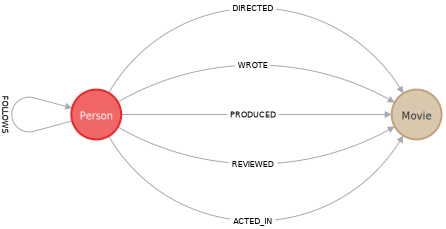
\includegraphics[width=0.8\linewidth,keepaspectratio]{neo4j62}
\end{center}	  


{\tiny (Ref: Introduction to cypher fundamentals  - neo4j)}

\end{frame}

%%%%%%%%%%%%%%%%%%%%%%%%%%%%%%%%%%%%%%%%%%%%%%%%%%%%%%%%%%%
\begin{frame}[fragile]\frametitle{Representation}


\begin{itemize}
\item Nodes are represented in round brackets \lstinline|() or (node variable name)|, similar to a circle on witheboard. An anonymous node \lstinline|()| represents one or more nodes during a query processing where there are no restrictions of the type of the node
\item Labels are used as type to group nodes and filter queries against the graph and is defined with a colon \lstinline|(:Label)|. A node can have zero or more labels for example \lstinline|(node), (node:Label), (node:Label1:Label2), (:Label), (:Label1:Label2)|.
\item Relationships are represented as arrow with its label in square bracket in between \lstinline|-[:RELATIONSHIP]->|
\item Aliases or variable names are  used to referred elements to later in the query defined by a name before a name like \lstinline|(node1:Label1)<-[relationship:RELATIONSHIP]-(node2:Label2)| where \lstinline|node1, node2| and \lstinline|relationship| are aliases.
\item he properties of a node are accessed using \lstinline|{variable}.{property_key}|, for example \lstinline|emil.name or movie.title|.
\end{itemize}

{\tiny (Ref: Learning Neo4j - Wabri Github)}


\end{frame}

%%%%%%%%%%%%%%%%%%%%%%%%%%%%%%%%%%%%%%%%%%%%%%%%%%%%%%%%%%%
\begin{frame}[fragile]\frametitle{Representation}


\begin{center}
\includegraphics[width=\linewidth,keepaspectratio]{neo4j63}
\end{center}	  


{\tiny (Ref: Introduction to cypher fundamentals  - neo4j)}

\end{frame}


%%%%%%%%%%%%%%%%%%%%%%%%%%%%%%%%%%%%%%%%%%%%%%%%%%%%%%%%%%%%%%%%%%%%%%%%%%%%%%%%%%
\begin{frame}[fragile]\frametitle{}
\begin{center}
{\Large Reading}
\end{center}
\end{frame}


%%%%%%%%%%%%%%%%%%%%%%%%%%%%%%%%%%%%%%%%%%%%%%%%%%%%%%%%%%%
\begin{frame}[fragile]\frametitle{Basic Syntax}

\begin{center}
\includegraphics[width=\linewidth,keepaspectratio]{neo4j9}
\end{center}	  


{\tiny (Ref: Introduction to Neo4j - a hands-on crash course  - neo4j)}

\end{frame}

%%%%%%%%%%%%%%%%%%%%%%%%%%%%%%%%%%%%%%%%%%%%%%%%%%%%%%%%%%%
\begin{frame}[fragile]\frametitle{Retrieval}


\begin{itemize}
\item Pattern specification for MATCH command, to retrieve data in graph.
\item Find and return person $p$ and movie $m$
\item First finds $p$ with given name, then goes to all relationships with given type and then finds $m$ which matches given title.
\end{itemize}


\begin{center}
\includegraphics[width=0.8\linewidth,keepaspectratio]{neo4j64}
\end{center}	  


{\tiny (Ref: Introduction to cypher fundamentals  - neo4j)}

\end{frame}

%%%%%%%%%%%%%%%%%%%%%%%%%%%%%%%%%%%%%%%%%%%%%%%%%%%%%%%%%%%
\begin{frame}[fragile]\frametitle{Retrieval}

WHERE can be used to add logical expression, which is not possible in MATCH

\begin{center}
\includegraphics[width=0.8\linewidth,keepaspectratio]{neo4j65}
\end{center}	  


{\tiny (Ref: Introduction to cypher fundamentals  - neo4j)}

\end{frame}



%%%%%%%%%%%%%%%%%%%%%%%%%%%%%%%%%%%%%%%%%%%%%%%%%%%%%%%%%%%
\begin{frame}[fragile]\frametitle{MATCH}

Retrieve nodes

\begin{center}
\includegraphics[width=\linewidth,keepaspectratio]{neo4j10}
\end{center}	  


{\tiny (Ref: Introduction to Neo4j - a hands-on crash course  - neo4j)}

\end{frame}

%%%%%%%%%%%%%%%%%%%%%%%%%%%%%%%%%%%%%%%%%%%%%%%%%%%%%%%%%%%
\begin{frame}[fragile]\frametitle{MATCH}

Retrieve nodes with properties

\begin{center}
\includegraphics[width=\linewidth,keepaspectratio]{neo4j11}
\end{center}	  


{\tiny (Ref: Introduction to Neo4j - a hands-on crash course  - neo4j)}

\end{frame}

%%%%%%%%%%%%%%%%%%%%%%%%%%%%%%%%%%%%%%%%%%%%%%%%%%%%%%%%%%%
\begin{frame}[fragile]\frametitle{MATCH}

Retrieve nodes with relationships

\begin{center}
\includegraphics[width=\linewidth,keepaspectratio]{neo4j12}
\end{center}	  


{\tiny (Ref: Introduction to Neo4j - a hands-on crash course  - neo4j)}

\end{frame}

%%%%%%%%%%%%%%%%%%%%%%%%%%%%%%%%%%%%%%%%%%%%%%%%%%%%%%%%%%%
\begin{frame}[fragile]\frametitle{Retrieval}


\begin{itemize}
\item Absence of a property can also be checked in WHERE clause
\item Partial matches are allowed using STARTS\_WITH, ENDS\_WITH keywords
\item String tests are case sensitive, so better to LOWER them.
\item Check presence IN a list
\end{itemize}


\begin{center}
\includegraphics[width=\linewidth,keepaspectratio]{neo4j66}

\includegraphics[width=\linewidth,keepaspectratio]{neo4j67}

\end{center}	  


{\tiny (Ref: Introduction to cypher fundamentals  - neo4j)}

\end{frame}

%%%%%%%%%%%%%%%%%%%%%%%%%%%%%%%%%%%%%%%%%%%%%%%%%%%%%%%%%%%
\begin{frame}[fragile]\frametitle{Exercise}

Write and execute a query to return all Movie titles in the graph that have a title that begins with "Life is". There may be titles that do not adhere to capitalization as such so you must ensure that all titles will match. That is, it will retrieve any case of the string, such as "Life is", "LIFE IS", "life is", "Life Is".

{\tiny (Ref: Intermediate Cypher - neo4j)}

\end{frame}

%%%%%%%%%%%%%%%%%%%%%%%%%%%%%%%%%%%%%%%%%%%%%%%%%%%%%%%%%%%
\begin{frame}[fragile]\frametitle{Solution}

\begin{lstlisting}
MATCH (m:Movie)
WHERE toLower(m.title) STARTS WITH "life is"
RETURN m.title
\end{lstlisting}	

\end{frame}

%%%%%%%%%%%%%%%%%%%%%%%%%%%%%%%%%%%%%%%%%%%%%%%%%%%%%%%%%%%
\begin{frame}[fragile]\frametitle{Exercise}

Write and execute a query to return the name of the person, their role, and the movie title where the role played by the actors or director had a value that included 'dog' (case-insensitive)? That is, the role could contain "Dog", "dog", or even "DOG".

{\tiny (Ref: Intermediate Cypher - neo4j)}

\end{frame}

%%%%%%%%%%%%%%%%%%%%%%%%%%%%%%%%%%%%%%%%%%%%%%%%%%%%%%%%%%%
\begin{frame}[fragile]\frametitle{Solution}

\begin{lstlisting}
MATCH (p:Person)-[r]->(m:Movie)
WHERE toLower(r.role) CONTAINS "dog"
RETURN p.name, r.role, m.title
\end{lstlisting}	

\end{frame}

%%%%%%%%%%%%%%%%%%%%%%%%%%%%%%%%%%%%%%%%%%%%%%%%%%%%%%%%%%%
\begin{frame}[fragile]\frametitle{Aggregates}

\begin{itemize}
\item No need to specify grouping key. There is no group-by statement. Other Aggregates are SUM, STDDEV, etc.
\item count(n) calculates the number of non-null occurrences of n. 
\item count(*) calculates the number of rows retrieved, including those with null values 
\item count() will implicit group by based upon the aggregation.
\end{itemize}

{\tiny (Ref: Learning Neo4j - Wabri Github)}


\begin{lstlisting}
// implicitly groups by p.name
MATCH (p.Person)-[:ACTED_IN]->(m:Movie)
RETURN p.name, count(*) AS numberOfMovies
\end{lstlisting}	

\end{frame}

%%%%%%%%%%%%%%%%%%%%%%%%%%%%%%%%%%%%%%%%%%%%%%%%%%%%%%%%%%%%%%%%%%%%%%%%%%%%%%%%%%
\begin{frame}\frametitle{Properties }

\begin{itemize}
\item Properties can be used to filter queries so that a subset of the graph is retrieved. \lstinline|CALL db.propertyKeys|
\item Nodes properties filtering \lstinline|MATCH (variable:Label {propertyKey1: propertyValue1, propertyKey2: propertyValue2}) RETURN variable|
\item In addition, with the RETURN clause, you can return property values from the retrieved nodes, rather than the nodes. \lstinline|MATCH (variable {property1: value}) RETURN variable.property2|
\end{itemize}


{\tiny (Ref: Learning Neo4j - Wabri Github)}
\end{frame}

%%%%%%%%%%%%%%%%%%%%%%%%%%%%%%%%%%%%%%%%%%%%%%%%%%%%%%%%%%%%%%%%%%%%%%%%%%%%%%%%%%
\begin{frame}\frametitle{Aliases }

\begin{itemize}
\item To customize the headings for a table containing property value it can be use aliases: \lstinline|MATCH (variable:Label {property1: value, property2: value}) RETURN variable.property2 AS alias1, variable.property3 AS alias2|
\item In the graph database we can specify aliases for the returned property values: \lstinline|MATCH (p:Person {born: 1970}) RETURN p.name AS name, p.born AS 'birth year'|
\end{itemize}


{\tiny (Ref: Learning Neo4j - Wabri Github)}
\end{frame}

%%%%%%%%%%%%%%%%%%%%%%%%%%%%%%%%%%%%%%%%%%%%%%%%%%%%%%%%%%%%%%%%%%%%%%%%%%%%%%%%%%
\begin{frame}\frametitle{Relationships}

The relationship can be specified with or without direction.

\begin{itemize}
\item \lstinline|() // a node|
\item \lstinline|()--() // 2 nodes have some type of relationship|
\item \lstinline|()-->() // the first node has a relationship to the second node|
\item \lstinline|()<--() // the second node has a relationship to the first node |
\end{itemize}

{\tiny (Ref: Learning Neo4j - Wabri Github)}
\end{frame}

%%%%%%%%%%%%%%%%%%%%%%%%%%%%%%%%%%%%%%%%%%%%%%%%%%%%%%%%%%%%%%%%%%%%%%%%%%%%%%%%%%
\begin{frame}\frametitle{Style recommendations}

\begin{itemize}
\item Node labels are CamelCase and begin with an upper-case letter, like Person or NetworkAddress.
\item Property keys, variables, parameters, aliases, and functions are camelCase and begin with a lower-case letter, like title or businessAddress.
\item Relationship type are in upper-case and can use the underscore, like ACTED\_IN or FOLLOWS.
\item Cypher keywords are upper-case, like MATCH or RETURN.
\item String constants are in single quotes, unless the string contains a quote or apostrophe, like 'The Matrix' or ``Somethings Gotta Give''.
\item Specify variables only when needed for use later in the cypher statement.
\item Place named nodes and relationships before anonymous nodes and relationships in the MATCH clauses when possible.
\item Specify anonymous relationships with \lstinline|-->, --, or <--|
\end{itemize}

{\tiny (Ref: Learning Neo4j - Wabri Github)}
\end{frame}

%%%%%%%%%%%%%%%%%%%%%%%%%%%%%%%%%%%%%%%%%%%%%%%%%%%%%%%%%%%%%%%%%%%%%%%%%%%%%%%%%%
\begin{frame}[fragile]\frametitle{Multiple Match patterns}

The MATCH clause includes a pattern specified by two paths separated by a comma:

\begin{lstlisting}
MATCH (a:Person)-[:ACTED_IN]->(m:Movie),
    (m:Movie)<-[:DIRECTED]-(d:Person)
WHERE m.released = 2000
RETURN a.name, m.title, d.name
\end{lstlisting}

\end{frame}

%%%%%%%%%%%%%%%%%%%%%%%%%%%%%%%%%%%%%%%%%%%%%%%%%%%%%%%%%%%%%%%%%%%%%%%%%%%%%%%%%%
\begin{frame}[fragile]\frametitle{Setting path variables}

It's possible to assign to a variable a path that can be reuse later in the same query or if it's needed to return that path:


\begin{lstlisting}
MATCH megPath = (meg:Person)-[:ACTED_IN]->(m:Movie)<-[:DIRECTED]-(d:Person),
    (other:Person)-[:ACTED_IN]->(m)
WHERE meg.name = 'Meg Ryan'
RETURN megPath
\end{lstlisting}

\end{frame}

%%%%%%%%%%%%%%%%%%%%%%%%%%%%%%%%%%%%%%%%%%%%%%%%%%%%%%%%%%%%%%%%%%%%%%%%%%%%%%%%%%
\begin{frame}[fragile]\frametitle{Varying length paths}

It's possible to assign to a variable a path that can be reuse later in the same query or if it's needed to return that path:


\begin{itemize}
\item Any graph that represents social networking, trees, or hierarchies will most likely have multiple paths of varying lengths.

\item To get this far you need to use this format \lstinline|(nodeA)-[:REALTYPE*<number_of_hops>]->(nodeB) or (nodeA)-[:REALTYPE*n..m]->(nodeB)| where n and m are the extremes of an interval.
\end{itemize}

{\tiny (Ref: Learning Neo4j - Wabri Github)}
\end{frame}

%%%%%%%%%%%%%%%%%%%%%%%%%%%%%%%%%%%%%%%%%%%%%%%%%%%%%%%%%%%%%%%%%%%%%%%%%%%%%%%%%%
\begin{frame}[fragile]\frametitle{Finding the shortest path}

A built-in function that you may find useful in a graph that has many ways of traversing the graph to get to the same node is the shortestPath() function. Using the shortest path between two nodes improves the performance of the query.

\begin{lstlisting}
MATCH p = shortestPath((m1:Movie)-[*]-(m2:Movie))
WHERE m1.title = 'A Few Good Men' AND
    m2.title = 'The Matrix'
RETURN p
\end{lstlisting}

\end{frame}

%%%%%%%%%%%%%%%%%%%%%%%%%%%%%%%%%%%%%%%%%%%%%%%%%%%%%%%%%%%%%%%%%%%%%%%%%%%%%%%%%%
\begin{frame}[fragile]\frametitle{Optional pattern matching}
This clause OPTIONAL MATCH is just like the MATCH but if no matches are found, this clause will use null for missing parts of the pattern. Here is an examples:

\begin{lstlisting}
MATCH (p:Person)
WHERE p.name STARTS WITH 'James'
OPTIONAL MATCH (p)-[r:REVIEWED]->(m:Movie)
RETURN p.name, type(r), m.title
\end{lstlisting}


\begin{center}
\includegraphics[width=0.4\linewidth,keepaspectratio]{neo4j83}
\end{center}	


{\tiny (Ref: Learning Neo4j - Wabri Github)}
\end{frame}

%%%%%%%%%%%%%%%%%%%%%%%%%%%%%%%%%%%%%%%%%%%%%%%%%%%%%%%%%%%%%%%%%%%%%%%%%%%%%%%%%%
\begin{frame}[fragile]\frametitle{Collecting results }

Cypher has a built-in function collect() that enables you to aggregate value into a list and the result will be a list called movies for Tom Cruise with the values ["Jerry Maguire", "Top Gun", "A Few Good Men"].

\begin{lstlisting}
MATCH (p:Person)-[:ACTED_IN]->(m:Movie)
WHERE p.name = 'Tom Cruise'
RETURN collect(m.title) AS `movies for Tom Cruise`
\end{lstlisting}


\end{frame}

%%%%%%%%%%%%%%%%%%%%%%%%%%%%%%%%%%%%%%%%%%%%%%%%%%%%%%%%%%%%%%%%%%%%%%%%%%%%%%%%%%
\begin{frame}[fragile]\frametitle{Exercise }

Write a query to return the number of movies a person directed.

What is the highest number of movies a director directed in our graph?


\end{frame}

%%%%%%%%%%%%%%%%%%%%%%%%%%%%%%%%%%%%%%%%%%%%%%%%%%%%%%%%%%%%%%%%%%%%%%%%%%%%%%%%%%
\begin{frame}[fragile]\frametitle{Solution}

\begin{lstlisting}
MATCH (d:Director)-[:DIRECTED]-(m)
RETURN d.name AS Director,
count(*) AS numMovies
ORDER BY numMovies DESC LIMIT 5
\end{lstlisting}

\end{frame}

%%%%%%%%%%%%%%%%%%%%%%%%%%%%%%%%%%%%%%%%%%%%%%%%%%%%%%%%%%%%%%%%%%%%%%%%%%%%%%%%%%
\begin{frame}[fragile]\frametitle{Exercise }

Write and execute a query to return the list of actors for each movie. Order and limit the results so that the movie with the largest cast is returned.

What movie had the largest list of actors? (Enter a case-sensitive string for the movie title.)

\end{frame}

%%%%%%%%%%%%%%%%%%%%%%%%%%%%%%%%%%%%%%%%%%%%%%%%%%%%%%%%%%%%%%%%%%%%%%%%%%%%%%%%%%
\begin{frame}[fragile]\frametitle{Solution}

\begin{lstlisting}
MATCH (a:Actor)-[:ACTED_IN]->(m:Movie)
RETURN m.title AS movie,
collect(a.name) AS cast,
size(collect(a.name)) AS num
ORDER BY num DESC LIMIT 1
\end{lstlisting}

\end{frame}

%%%%%%%%%%%%%%%%%%%%%%%%%%%%%%%%%%%%%%%%%%%%%%%%%%%%%%%%%%%%%%%%%%%%%%%%%%%%%%%%%%
\begin{frame}[fragile]\frametitle{List comprehension}

Create a list by evaluating an expression that tests for list inclusion.

\begin{lstlisting}
MATCH (m:Movie)
RETURN m.title as movie,
[x IN m.countries WHERE x = 'USA' OR x = 'Germany']
AS country LIMIT 500
\end{lstlisting}


\end{frame}

%%%%%%%%%%%%%%%%%%%%%%%%%%%%%%%%%%%%%%%%%%%%%%%%%%%%%%%%%%%%%%%%%%%%%%%%%%%%%%%%%%
\begin{frame}[fragile]\frametitle{Pattern comprehension}

\begin{itemize}
\item To create lists without changing the cardinality of the query. It behaves like an OPTIONAL MATCH combined with collect().
\item Specify the list with the square braces to include the pattern followed by the pipe character to then specify what value will be placed in the list from the pattern.

\lstinline{[<pattern> | value]}
\item This query returns the movies released in 2015. Each row contains the title of the movie, the list of director names, and the list of actor names.
\end{itemize}

\begin{lstlisting}
MATCH (m:Movie)
WHERE m.year = 2015
RETURN m.title,
[(dir:Person)-[:DIRECTED]->(m) | dir.name] AS directors,
[(actor:Person)-[:ACTED_IN]->(m) | actor.name] AS actors
\end{lstlisting}


\end{frame}

%%%%%%%%%%%%%%%%%%%%%%%%%%%%%%%%%%%%%%%%%%%%%%%%%%%%%%%%%%%%%%%%%%%%%%%%%%%%%%%%%%
\begin{frame}[fragile]\frametitle{Pattern comprehension}

Using pattern comprehension to create a list where we specify a filter for the pattern.

\begin{lstlisting}
MATCH (a:Person {name: 'Tom Hanks'})
RETURN [(a)-->(b:Movie)
WHERE b.title CONTAINS "Toy" | b.title + ": " + b.year]
AS movies
\end{lstlisting}


\end{frame}

%%%%%%%%%%%%%%%%%%%%%%%%%%%%%%%%%%%%%%%%%%%%%%%%%%%%%%%%%%%%%%%%%%%%%%%%%%%%%%%%%%
\begin{frame}[fragile]\frametitle{Working with maps}

\begin{itemize}
\item A Cypher map is list of key/value pairs where each element of the list is of the format 'key': value. 
\item A node or relationship can have a property that is a map.
\item or example, a map of months and the number of days per month could be: \lstinline|{Jan: 31, Feb: 28, Mar: 31, Apr: 30 , May: 31, Jun: 30 , Jul: 31, Aug: 31, Sep: 30, Oct: 31, Nov: 30, Dec: 31}|
\item Using this map, we can return the value for one of its elements. Here we use the key, 'Feb' to access its value.

\item you can return a list of keys of a map as follows:
\end{itemize}

\begin{lstlisting}
RETURN {Jan: 31, Feb: 28, Mar: 31, Apr: 30 ,
May: 31, Jun: 30 , Jul: 31, Aug: 31, Sep: 30,
Oct: 31, Nov: 30, Dec: 31}['Feb'] AS daysInFeb

RETURN keys({Jan: 31, Feb: 28, Mar: 31, Apr: 30 ,
May: 31, Jun: 30 ,Jul: 31, Aug: 31, Sep: 30,
Oct: 31, Nov: 30, Dec: 31}) AS months
\end{lstlisting}


\end{frame}

%%%%%%%%%%%%%%%%%%%%%%%%%%%%%%%%%%%%%%%%%%%%%%%%%%%%%%%%%%%%%%%%%%%%%%%%%%%%%%%%%%
\begin{frame}[fragile]\frametitle{Working with dates and times}

Create some date node

\begin{lstlisting}
MERGE (x:Test {id: 1})
SET
x.date = date(),
x.datetime = datetime(),
x.timestamp = timestamp(),
x.date1 = date('2022-04-08'),
x.date2 = date('2022-09-20'),
x.datetime1 = datetime('2022-02-02T15:25:33'),
x.datetime2 = datetime('2022-02-02T22:06:12')
RETURN x
\end{lstlisting}


\end{frame}

%%%%%%%%%%%%%%%%%%%%%%%%%%%%%%%%%%%%%%%%%%%%%%%%%%%%%%%%%%%%%%%%%%%%%%%%%%%%%%%%%%
\begin{frame}[fragile]\frametitle{Working with dates and times}

\begin{itemize}
\item Write a query to retrieve this Test node and calculate the number of days between date1 and date2.
\item Write a query to retrieve this Test node and calculate the number of minutes between datetime1 and datetime2.
\end{itemize}

\begin{lstlisting}
// calculate the duration
MATCH (x:Test)
RETURN duration.inDays(x.date1,x.date2).days

// calculate the duration in minutes
MATCH (x:Test)
RETURN duration.between(x.datetime1,x.datetime2).minutes
\end{lstlisting}


\end{frame}


%%%%%%%%%%%%%%%%%%%%%%%%%%%%%%%%%%%%%%%%%%%%%%%%%%%%%%%%%%%%%%%%%%%%%%%%%%%%%%%%%%
\begin{frame}[fragile]\frametitle{Additional processing using WITH}

\begin{itemize}
\item WITH defines or re-defines scope of the variable
\item With the WITH clause it's possible to perform intermediate processing of data flow operations.
\item The WITH clause removes variables from scope for the RETURN clause so you must add them back to the scope.
\item This example return the actors name only if they acted on 2 or 3 movies, with a reference of the numbers of the films and a list of that.
\item Using WITH as you are scoping processing, step by step, its called Pipelining.
\end{itemize}

\begin{lstlisting}
WITH 'toy story' as mt, and 'Tom Hanks' AS actorName
MATCH (a:Person)-[:ACTED_IN]->(m:Movie)
WHERE p.name = actorName AND toLower(m.title) CONTAINS mt
RETURN m.title AS movies

MATCH (a:Person)-[:ACTED_IN]->(m:Movie)
WITH a, count(a) AS numMovies, collect(m.title) AS movies
WHERE numMovies > 1 AND numMovies < 4
RETURN a.name, numMovies, movies
\end{lstlisting}

\end{frame}

%%%%%%%%%%%%%%%%%%%%%%%%%%%%%%%%%%%%%%%%%%%%%%%%%%%%%%%%%%%%%%%%%%%%%%%%%%%%%%%%%%
\begin{frame}[fragile]\frametitle{Additional processing using WITH}

Adding a WITH clause that customizes the data returned for each Movie node to include:
\begin{itemize}
\item title
\item imdbRating
\item List of actor names
\item List of Genre names
\end{itemize}

\begin{lstlisting}
MATCH (n:Movie)
WHERE n.imdbRating IS NOT NULL AND n.poster IS NOT NULL
WITH n {
  .title,
  .imdbRating,
  actors: [ (n)<-[:ACTED_IN]-(p) | p { tmdbId:p.imdbId, .name } ],
  genres: [ (n)-[:IN_GENRE]->(g) | g {.name}]
}
ORDER BY n.imdbRating DESC
LIMIT 4
RETURN collect(n)
\end{lstlisting}

\end{frame}

%%%%%%%%%%%%%%%%%%%%%%%%%%%%%%%%%%%%%%%%%%%%%%%%%%%%%%%%%%%%%%%%%%%%%%%%%%%%%%%%%%
\begin{frame}[fragile]\frametitle{Additional processing using WITH}

Remember to name all expressions with an alias in a WITH that are not simple variables. This is a simple query to retrieve all the actor that are acted in at least 5 movies and if they also directed a movie than return the name of that movie.


\begin{lstlisting}
MATCH (p:Person)
WITH p, size((p)-[:ACTED_IN]->(:Movie)) as movies
WHERE movies>=5
OPTIONAL MATCH (p)-[:DIRECTED]->(m:Movie)
RETURN p.name, m.title

\end{lstlisting}


\begin{center}
\includegraphics[width=0.4\linewidth,keepaspectratio]{neo4j84}
\end{center}	


{\tiny (Ref: Learning Neo4j - Wabri Github)}
\end{frame}

%%%%%%%%%%%%%%%%%%%%%%%%%%%%%%%%%%%%%%%%%%%%%%%%%%%%%%%%%%%%%%%%%%%%%%%%%%%%%%%%%%
\begin{frame}[fragile]\frametitle{Eliminating duplication}

To eliminating duplicated results it can be used the DISTINCT keyword



\begin{lstlisting}
MATCH (gene:Person)-[:ACTED_IN]->(movie:Movie)
WHERE gene.name = 'Gene Hackman'
OPTIONAL MATCH
    (other:Person)-[:ACTED_IN]->(movie),
    (dir:Person)-[:DIRECTED]->(movie)
WITH
    movie,
    collect(other.name) AS Actors,
    collect(DISTINCT dir.name) AS Directors
RETURN
    movie.title AS `Title of movie`,
    Actors AS `Co-Actors`,
    Directors

\\ can be use in several uses, like this:

MATCH (p:Person)-[:DIRECTED | :ACTED_IN]->(m:Movie)
WHERE p.name = 'Tom Hanks'
WITH DISTINCT m
RETURN m.released, m.title
\end{lstlisting}

\end{frame}

%%%%%%%%%%%%%%%%%%%%%%%%%%%%%%%%%%%%%%%%%%%%%%%%%%%%%%%%%%%%%%%%%%%%%%%%%%%%%%%%%%
\begin{frame}[fragile]\frametitle{Ordering result}

If you want the results to be sorted, you specify the expression to use for the sort usign the ORDER BY keyword and whether you want the order to be descending using the DESC keyword.


\begin{lstlisting}
MATCH (p:Person)-[:DIRECTED | :ACTED_IN]->(m:Movie)
WHERE p.name = 'Tom Hanks' AND m.released >= 2000
RETURN m.released, collect(DISTINCT m.title) AS movies ORDER BY m.released DESC
//
\end{lstlisting}

\begin{center}
\includegraphics[width=0.4\linewidth,keepaspectratio]{neo4j85}
\end{center}	  


{\tiny (Ref: Learning Neo4j - Wabri Github)}
\end{frame}

%%%%%%%%%%%%%%%%%%%%%%%%%%%%%%%%%%%%%%%%%%%%%%%%%%%%%%%%%%%%%%%%%%%%%%%%%%%%%%%%%%
\begin{frame}[fragile]\frametitle{Exercise}

Write and execute a query to return the movie titles where they are ordered from the highest to the lowest imdbRating value. In your query, only return movies that have a value for the imdbRating property.


{\tiny (Ref: Intermediate Cypher - neo4j)}
\end{frame}

%%%%%%%%%%%%%%%%%%%%%%%%%%%%%%%%%%%%%%%%%%%%%%%%%%%%%%%%%%%%%%%%%%%%%%%%%%%%%%%%%%
\begin{frame}[fragile]\frametitle{Solution}

\begin{lstlisting}
MATCH (m:Movie)
WHERE m.imdbRating IS NOT NULL
RETURN m.title as title, m.imdbRating as rating
ORDER BY m.imdbRating DESC
\end{lstlisting}

\end{frame}

%%%%%%%%%%%%%%%%%%%%%%%%%%%%%%%%%%%%%%%%%%%%%%%%%%%%%%%%%%%%%%%%%%%%%%%%%%%%%%%%%%
\begin{frame}[fragile]\frametitle{Limiting the number of results}

Although you can filter queries to reduce the number of results returned, you may also want to limit the number of results. This is useful if you have very large result sets and you only need to see the beginning or end of a set of ordered results. LIMIT is the right choice to do something like this.

\begin{lstlisting}
MATCH (m:Movie)
RETURN m.title as title, m.released as year
ORDER BY m.released DESC
LIMIT 10
\end{lstlisting}


\end{frame}

%%%%%%%%%%%%%%%%%%%%%%%%%%%%%%%%%%%%%%%%%%%%%%%%%%%%%%%%%%%%%%%%%%%%%%%%%%%%%%%%%%
\begin{frame}[fragile]\frametitle{Switch/Case Statement}

Returning results conditionally

\begin{lstlisting}
MATCH (m:Movie)<-[:ACTED_IN]-(p:Person)
WHERE p.name = 'Henry Fonda'
RETURN m.title AS movie,
CASE
WHEN m.year < 1940 THEN 'oldies'
WHEN 1940 <= m.year < 1950 THEN 'forties'
WHEN 1950 <= m.year < 1960 THEN 'fifties'
WHEN 1960 <= m.year < 1970 THEN 'sixties'
WHEN 1970 <= m.year < 1980 THEN 'seventies'
WHEN 1980 <= m.year < 1990 THEN 'eighties'
WHEN 1990 <= m.year < 2000 THEN 'nineties'
ELSE  'two-thousands'
END
AS timeFrame
\end{lstlisting}
\end{frame}

%%%%%%%%%%%%%%%%%%%%%%%%%%%%%%%%%%%%%%%%%%%%%%%%%%%%%%%%%%%%%%%%%%%%%%%%%%%%%%%%%%
\begin{frame}[fragile]\frametitle{List}

A Cypher map is list of key/value pairs where each element of the list is of the format key: value.

It's possible to collect values for a list during a query and with this it's possible to sort by the size of the list using the size() function as follows:

\begin{lstlisting}
MATCH (a:Person)-[:ACTED_IN]->(m:Movie)
WITH m, count(m) AS numCast, collect(a.name) AS cast
RETURN m.title, cast, numCast
ORDER BY size(cast)
\end{lstlisting}


\end{frame}



%%%%%%%%%%%%%%%%%%%%%%%%%%%%%%%%%%%%%%%%%%%%%%%%%%%%%%%%%%%%%%%%%%%%%%%%%%%%%%%%%%
\begin{frame}[fragile]\frametitle{Unwinding lists}

There my be some situations where you want to perform the opposite of collecting results, but rather separate the lists into separate rows. This functionality is done using the unwind clause.

Here is an example where we create a list with three elements, unwind the list and then return the values. Since there are three elements, three rows are returned with the values:

\begin{lstlisting}
WITH [1, 2, 3] AS list
UNWIND list AS row
RETURN row, list
//
\end{lstlisting}


\begin{center}
\includegraphics[width=0.2\linewidth,keepaspectratio]{neo4j86}
\end{center}	 

The unwind clause is frequently used when importing data into a graph.

 

{\tiny (Ref: Learning Neo4j - Wabri Github)}
\end{frame}

%%%%%%%%%%%%%%%%%%%%%%%%%%%%%%%%%%%%%%%%%%%%%%%%%%%%%%%%%%%%%%%%%%%%%%%%%%%%%%%%%%
\begin{frame}[fragile]\frametitle{Dates}

Cypher has a built-in date() function, as well as other temporal values and functions that you can use to calculate temporal values. You use a combination of numeric, temporal, spatial, list and string functions to calculate values that are useful to your application.

For example we want to calculate all the age value of the actors given the born year:

\begin{lstlisting}
MATCH (actor:Person)-[:ACTED_IN]->(:Movie)
WHERE exists(actor.born)
WITH DISTINCT actor, date().year - actor.born AS age
RETURN actor.name, age AS `age today`
ORDER BY actor.born DESC
\end{lstlisting}

\end{frame}





%%%%%%%%%%%%%%%%%%%%%%%%%%%%%%%%%%%%%%%%%%%%%%%%%%%%%%%%%%%%%%%%%%%%%%%%%%%%%%%%%%
\begin{frame}[fragile]\frametitle{Anchors}

\begin{itemize}
\item Anchor node is the one from which fewest number of nodes need to be traversed
\item Persons are anchor nodes as there are 19047 persons but 28863 movies
\item In case there is filter, which reduces the search space, becomes anchor
\end{itemize}

\begin{lstlisting}
PROFILE MATCH (p:Person)-[:ACTED_IN]->(m)
RETURN p.name, m.title LIMIT 10

PROFILE MATCH (p:Person)-[:ACTED_IN]->(m)
WHERE p.name = 'Eminem"
RETURN p.name, m.title LIMIT 10
\end{lstlisting}



\end{frame}

%%%%%%%%%%%%%%%%%%%%%%%%%%%%%%%%%%%%%%%%%%%%%%%%%%%%%%%%%%%
\begin{frame}[fragile]\frametitle{Multiple Anchors}
There can be multiple answers where WHERE clauses are specified. Profile diagram shows them as index

\begin{lstlisting}
PROFILE MATCH (p1:Person)-[:ACTED_IN]->(m1), (p2:Person)-[:ACTED_IN]->(m2)
WHERE p1.name = 'Tom Hanks" AND p2.name = "Meg Ryan" AND m1 = m2
RETURN m.title


\end{lstlisting}

\begin{center}
\includegraphics[width=\linewidth,keepaspectratio]{neo4j90}
\end{center}	  

\end{frame}


%%%%%%%%%%%%%%%%%%%%%%%%%%%%%%%%%%%%%%%%%%%%%%%%%%%%%%%%%%%
\begin{frame}[fragile]\frametitle{Traversal}

\begin{itemize}
\item \lstinline|shortestPath()| finds that between two nodes
\item \lstinline|-[*]-| means regardless of relationship type
\item If you specify relationship types, typically path becomes longer
\end{itemize}


\begin{lstlisting}
MATCH p = shortestPath((p1:Person)-[*]-(p2:Person))
WHERE p1.name = "Eminem" AND p2.name = "Charlton Heston"
RETURN p


\end{lstlisting}

\begin{center}
\includegraphics[width=\linewidth,keepaspectratio]{neo4j91}
\end{center}	  
\end{frame}


%%%%%%%%%%%%%%%%%%%%%%%%%%%%%%%%%%%%%%%%%%%%%%%%%%%%%%%%%%%
\begin{frame}[fragile]\frametitle{Limiting Hops}

Between 1 to 6 hops


\begin{lstlisting}
MATCH (p:Person)-[:ACTED_IN*1..6]-(others:Person)
WHERE p.name = 'Tom Hanks'
RETURN  others.name
\end{lstlisting}

 
\end{frame}



%%%%%%%%%%%%%%%%%%%%%%%%%%%%%%%%%%%%%%%%%%%%%%%%%%%%%%%%%%%
\begin{frame}[fragile]\frametitle{Limiting Hops}

\begin{center}
\includegraphics[width=\linewidth,keepaspectratio]{neo4j92}
\end{center}	  
\end{frame}



%%%%%%%%%%%%%%%%%%%%%%%%%%%%%%%%%%%%%%%%%%%%%%%%%%%%%%%%%%%
\begin{frame}[fragile]\frametitle{Complex Example}
A Social Recommendation

\begin{center}
\includegraphics[width=\linewidth,keepaspectratio]{neo4j15}
\end{center}	  


{\tiny (Ref: Introduction to Neo4j and Graph Databases
 - M David Allen)}

\end{frame}



%%%%%%%%%%%%%%%%%%%%%%%%%%%%%%%%%%%%%%%%%%%%%%%%%%%%%%%%%%%
\begin{frame}[fragile]\frametitle{Complex Example}
What are the top 10 jobs for me, that are same location as I am in and also for which I have necessary qualifications?

\begin{center}
\includegraphics[width=\linewidth,keepaspectratio]{neo4j27}
\end{center}	    



{\tiny (Ref: Secret Sauce of Neo4j: Modeling and Querying Graphs
 - Max De Marzi )}

\end{frame}

%%%%%%%%%%%%%%%%%%%%%%%%%%%%%%%%%%%%%%%%%%%%%%%%%%%%%%%%%%%
\begin{frame}[fragile]\frametitle{Answer}

Partial sub-graph match

\begin{center}
\includegraphics[width=\linewidth,keepaspectratio]{neo4j28}
\end{center}	    


{\tiny (Ref: Secret Sauce of Neo4j: Modeling and Querying Graphs
 - Max De Marzi )}

\end{frame}


%%%%%%%%%%%%%%%%%%%%%%%%%%%%%%%%%%%%%%%%%%%%%%%%%%%%%%%%%%%%%%%%%%%%%%%%%%%%%%%%%%
\begin{frame}\frametitle{Example Data Model : Movies}

\begin{center}
\includegraphics[width=0.8\linewidth,keepaspectratio]{neo4j89}
\end{center}	

{\tiny (Ref: ``Intermediate Cypher - Graph Academy neo4j)}
\end{frame}

%%%%%%%%%%%%%%%%%%%%%%%%%%%%%%%%%%%%%%%%%%%%%%%%%%%%%%%%%%%%%%%%%%%%%%%%%%%%%%%%%%
\begin{frame}[fragile]\frametitle{Examples}

Find all Tom Hanks movies from 2013

\begin{lstlisting}
MATCH (p:Person-[:ACTED_IN]->(m:Movie)
WHERE p.name = "Tom Hanks"
AND m.year = 2013
RETURN m.title
\end{lstlisting}	

\end{frame}

%%%%%%%%%%%%%%%%%%%%%%%%%%%%%%%%%%%%%%%%%%%%%%%%%%%%%%%%%%%%%%%%%%%%%%%%%%%%%%%%%%
\begin{frame}[fragile]\frametitle{Examples}

Find all folks born before 1922 and still alive

\begin{lstlisting}
MATCH (p:Person)
WHERE p.died IS NULL
AND p.born.year <= 1922
RETURN p.name, p.born, p.died
\end{lstlisting}	

\end{frame}

%%%%%%%%%%%%%%%%%%%%%%%%%%%%%%%%%%%%%%%%%%%%%%%%%%%%%%%%%%%%%%%%%%%%%%%%%%%%%%%%%%
\begin{frame}[fragile]\frametitle{Examples}

Find all folks born after 1960 and are Actors and Directors both

\begin{lstlisting}
MATCH (p:Person)
WHERE p.born.year > 1960
AND p:Actor
AND p:Director
RETURN p.name, p.born, labels(p)
\end{lstlisting}	

\end{frame}

%%%%%%%%%%%%%%%%%%%%%%%%%%%%%%%%%%%%%%%%%%%%%%%%%%%%%%%%%%%%%%%%%%%%%%%%%%%%%%%%%%
\begin{frame}[fragile]\frametitle{Exercise}

Write a query to return all Movie nodes in the graph that do not have a tmdbId property.


{\tiny (Ref: ``Intermediate Cypher - Graph Academy neo4j)}
\end{frame}

%%%%%%%%%%%%%%%%%%%%%%%%%%%%%%%%%%%%%%%%%%%%%%%%%%%%%%%%%%%%%%%%%%%%%%%%%%%%%%%%%%
\begin{frame}[fragile]\frametitle{Solution}


\begin{lstlisting}
MATCH (m:Movie)
WHERE m.tmdbId IS NULL
RETURN count(m)
\end{lstlisting}	

\end{frame}


%%%%%%%%%%%%%%%%%%%%%%%%%%%%%%%%%%%%%%%%%%%%%%%%%%%%%%%%%%%%%%%%%%%%%%%%%%%%%%%%%%
\begin{frame}[fragile]\frametitle{Exercise}

Write and execute a query to return people who both acted in and directed a movie released in the German language.

{\tiny (Ref: ``Intermediate Cypher - Graph Academy neo4j)}
\end{frame}

%%%%%%%%%%%%%%%%%%%%%%%%%%%%%%%%%%%%%%%%%%%%%%%%%%%%%%%%%%%%%%%%%%%%%%%%%%%%%%%%%%
\begin{frame}[fragile]\frametitle{Solution}

\begin{lstlisting}
MATCH (p:Director)-[:DIRECTED]->(m:Movie)<-[:ACTED_IN]-(p)
WHERE "German" IN m.languages
RETURN count(DISTINCT p.name)
\end{lstlisting}	


\end{frame}


%%%%%%%%%%%%%%%%%%%%%%%%%%%%%%%%%%%%%%%%%%%%%%%%%%%%%%%%%%%%%%%%%%%%%%%%%%%%%%%%%%
\begin{frame}[fragile]\frametitle{}
\begin{center}
{\Large Writing}
\end{center}
\end{frame}



%%%%%%%%%%%%%%%%%%%%%%%%%%%%%%%%%%%%%%%%%%%%%%%%%%%%%%%%%%%
\begin{frame}[fragile]\frametitle{Nodes}

\begin{itemize}
\item MERGE: Creates a new node if not present already. All subsequent calls do not do anything as node with said properties is already present.

\item CREATE: Will create multiple nodes even if nodes with similar properties are present already
\end{itemize}

\begin{center}
\includegraphics[width=0.8\linewidth,keepaspectratio]{neo4j68}
\end{center}	  


{\tiny (Ref: Introduction to cypher fundamentals  - neo4j)}

\end{frame}

%%%%%%%%%%%%%%%%%%%%%%%%%%%%%%%%%%%%%%%%%%%%%%%%%%%%%%%%%%%
\begin{frame}[fragile]\frametitle{Nodes}


\begin{center}
\includegraphics[width=\linewidth,keepaspectratio]{neo4j13}
\end{center}	  


{\tiny (Ref: Introduction to Neo4j - a hands-on crash course  - neo4j)}

\end{frame}


%%%%%%%%%%%%%%%%%%%%%%%%%%%%%%%%%%%%%%%%%%%%%%%%%%%%%%%%%%%
\begin{frame}[fragile]\frametitle{Relationships}

\begin{itemize}
\item First get two existing nodes between which a relationship needs to be created.
\item Same MERGE logic is there for Relationships as well.
item Relationship type must begin with ':'
\end{itemize}

\begin{center}
\includegraphics[width=0.8\linewidth,keepaspectratio]{neo4j69}
\end{center}	  


{\tiny (Ref: Introduction to cypher fundamentals  - neo4j)}

\end{frame}

%%%%%%%%%%%%%%%%%%%%%%%%%%%%%%%%%%%%%%%%%%%%%%%%%%%%%%%%%%%
\begin{frame}[fragile]\frametitle{Properties}

\begin{itemize}
\item Use SET to set new or existing properties
\item It can be used for both Nodes and Relationships
\item Use REMOVE to remove a property. (it should not be a primary key though)
\end{itemize}

\begin{center}
\includegraphics[width=0.5\linewidth,keepaspectratio]{neo4j70}
\end{center}	  


{\tiny (Ref: Introduction to cypher fundamentals  - neo4j)}

\end{frame}


%%%%%%%%%%%%%%%%%%%%%%%%%%%%%%%%%%%%%%%%%%%%%%%%%%%%%%%%%%%
\begin{frame}[fragile]\frametitle{Constrains}
We add a uniqueness constraint to the graph by creating a constraint that asserts that a particular node property is unique in the graph for a particular type of node.

\begin{lstlisting}
// to ensure uniqueness and fast lookups
CREATE CONSTRAINT ON (label:Label)
ASSERT label.property IS UNIQUE

// This statement will fail if the graph already has multiple Movie nodes with the same value for the title property.

// We can also create a constraint on properties of relationships, its not necessary to define the direction of the relationship:

CREATE CONSTRAINT ON ()-[rel:REVIEWED]-() ASSERT exists(rel.rating)
\end{lstlisting}	  


\end{frame}

%%%%%%%%%%%%%%%%%%%%%%%%%%%%%%%%%%%%%%%%%%%%%%%%%%%%%%%%%%%
\begin{frame}[fragile]\frametitle{Conditionals}

\begin{itemize}
\item ON CREATE will do the SET at the time of creation, ie first time when the node is created. There ON MATCH wont run.
\item Next time, when the whole code is executed again, ON CRETAE wont run, but ON MATCH will.
\end{itemize}

\begin{center}
\includegraphics[width=0.8\linewidth,keepaspectratio]{neo4j71}
\end{center}	  


{\tiny (Ref: Introduction to cypher fundamentals  - neo4j)}
 

\end{frame}

%%%%%%%%%%%%%%%%%%%%%%%%%%%%%%%%%%%%%%%%%%%%%%%%%%%%%%%%%%%
\begin{frame}[fragile]\frametitle{Delete}

\begin{itemize}
\item Just get the reference to the object and delete it.
\item It can be a Node (if dangling) or a Relationship.
\item DETACH DELETE removes all relationships from the node and then DELETEs it.
\item To delete all nodes, just say \lstinline|MATCH (n) DETACH DELETE n|
\end{itemize}

\begin{center}
\includegraphics[width=0.8\linewidth,keepaspectratio]{neo4j72}
\end{center}	  


{\tiny (Ref: Introduction to cypher fundamentals  - neo4j)}
 

\end{frame}


%%%%%%%%%%%%%%%%%%%%%%%%%%%%%%%%%%%%%%%%%%%%%%%%%%%%%%%%%%%%%%%%%%%%%%%%%%%%%%%%%%
\begin{frame}[fragile]\frametitle{Parameters}

\begin{itemize}
\item In the Cypher statements, a parameter name begins with the \$ symbol.
\item At runtime, if the parameter \$actorName has a value, it will be used in the Cypher statement when it runs in the graph engine.
\item In Neo4j Browser to set values of parameters we can use the command :param:
\item \lstinline|:param actorName => 'Tom Hanks'|
\end{itemize}

\begin{lstlisting}
MATCH (p:Person)-[:ACTED_IN]->(m:Movie)
WHERE p.name = $actorName
RETURN m.released, m.title
ORDER BY m.released DESC
\end{lstlisting}

\end{frame}

%%%%%%%%%%%%%%%%%%%%%%%%%%%%%%%%%%%%%%%%%%%%%%%%%%%%%%%%%%%%%%%%%%%%%%%%%%%%%%%%%%
\begin{frame}[fragile]\frametitle{Multiple MATCH}

\begin{itemize}
\item First MATCH gets a subset of ACTED relations tuples; checks years
\item Within them, finds Person with DIRECTED
\item Generally, first sample has performance as single pattern is better.
\item OPTIONAL MATCH if no match is found it will use nulls for missing parts of the pattern. .
\end{itemize}

\begin{lstlisting}
MATCH (a:Person)-[:ACTED_IN]->(m:Movie)
WHERE m.year > 2000
MATCH (m)-[:DIRECTED]->(d:Person)
RETURN a.name, m.title, d.name

MATCH (a:Person)-[:ACTED_IN]->(m:Movie), (m)-[:DIRECTED]->(d:Person)
WHERE m.year > 2000
RETURN a.name, m.title, d.name
\end{lstlisting}

\end{frame}

%%%%%%%%%%%%%%%%%%%%%%%%%%%%%%%%%%%%%%%%%%%%%%%%%%%%%%%%%%%%%%%%%%%%%%%%%%%%%%%%%%
\begin{frame}[fragile]\frametitle{Performance}

\begin{itemize}
\item There could be multiple ways to get the answer
\item Difference is the performance, which depends on how much of graph traversal is needed
\item \lstinline|exists| is checked for all movies Tom Hanks has acted in. ie. 38 (find it using PROFILE)
\item Next example below is a better query as it has only 2 rows in between.
\item But sometimes there may not be a choice but to use `exists`, such as find movies where Tom Hanks has acted but not directed.
\end{itemize}

\begin{lstlisting}
MATCH (p:Person)-[:ACTED_IN]->(m:Movie)
WHERE p.name = "Tom Hanks"
AND exists {(p)-[:DIRECTED]->(m)}
RETURN p.name, labels(p), m.title

MATCH (p:Person)-[:ACTED_IN]->(m:Movie)<-[DIRECTED]-(p)
WHERE p.name = "Tom Hanks"
RETURN m.title
\end{lstlisting}

\end{frame}


%%%%%%%%%%%%%%%%%%%%%%%%%%%%%%%%%%%%%%%%%%%%%%%%%%%%%%%%%%%%%%%%%%%%%%%%%%%%%%%%%%
\begin{frame}[fragile]\frametitle{Explain Profile}

There are two Cypher keywords to use as prefix with a Cypher statement to analyze a query:
\begin{itemize}
\item EXPLAIN provides estimates of the graph engine processing that will occur, but does not execute the statement.
\item PROFILE provides real profiling information for what has occurred in the graph engine during the query and executes the statement.
\item This query return the phases of the Cypher execution, it can be possible to examine what code is expected to run. Each phase of the query presents an estimante of the number of rows expected to be returned.
\end{itemize}

\begin{lstlisting}
EXPLAIN
MATCH (p:Person)-[:ACTED_IN]->(m:Movie)
WHERE p.name = $actorName AND
      m.released < $year
RETURN p.name, m.title, m.released

\end{lstlisting}

\end{frame}


%%%%%%%%%%%%%%%%%%%%%%%%%%%%%%%%%%%%%%%%%%%%%%%%%%%%%%%%%%%%%%%%%%%%%%%%%%%%%%%%%%
\begin{frame}[fragile]\frametitle{Profile}

\begin{itemize}
\item For a better metric for analyzing how the Cypher statement will run is needed to run the PROFILE prefix keyword which runs the statement and gives the run-time performance metrics.
\item This query above show the cache hits and most importantly the number of times that the engine accessed the database (db hints). This is the metric that will affect the performance of the Cypher statement at run-time.
\end{itemize}

\begin{lstlisting}
PROFILE
MATCH (p:Person)-[:ACTED_IN]->(m:Movie)
WHERE p.name = $actorName AND
      m.released < $year
RETURN p.name, m.title, m.released
\end{lstlisting}



\end{frame}


%%%%%%%%%%%%%%%%%%%%%%%%%%%%%%%%%%%%%%%%%%%%%%%%%%%%%%%%%%%
\begin{frame}[fragile]\frametitle{Managing indexes}
The uniqueness and node key constraints are essentially single-property and composite indexes respectively. Indexes are used to improve initial node lookup performance, but they require additional storage in the graph to maintain and also add to the cost of creating or modifying property values that are indexed. Indexes store redundant data that points to nodes with the specific property value or values. Unlike SQL, there is no such thing as a primary key in Neo4j, but nodes can have multiple properties that must be unique. This are single-property indexes used:



\begin{itemize}
\item Equality checks: $=$
\item Range comparisons: $>,>=,<, <=$
\item List membership: IN
\item String comparisons: STARTS WITH, ENDS WITH, CONTAINS
\item Existence checks: exists()
\item Spatial distance searches: distance()
\item Spatial bounding searches: point()
\end{itemize}

Composite indexes are used only for equality checks and list membership.



{\tiny (Ref: Learning Neo4j - Wabri Github)}

\end{frame}

%%%%%%%%%%%%%%%%%%%%%%%%%%%%%%%%%%%%%%%%%%%%%%%%%%%%%%%%%%%
\begin{frame}[fragile]\frametitle{Managing indexes}
\begin{itemize}
\item The index for a property of a node can greatly reduce the number of nodes that the engine needs to visit in oredr to satisy a query.
\item The graph engine will find the pointers to all nodes that satisfy the query without having to visit all of the nodes:
\end{itemize}


\begin{lstlisting}
MATCH (m:Movie)
WHERE 1990 < m.released < 2000
SET m.videoFormat = 'DVD'
\end{lstlisting}

\end{frame}

%%%%%%%%%%%%%%%%%%%%%%%%%%%%%%%%%%%%%%%%%%%%%%%%%%%%%%%%%%%
\begin{frame}[fragile]\frametitle{From relational to graph}
To convert a relational database into a graph database with one step you can use the ETL tool (Extract Transform Load) $->$ Neo4J ETL

In Cypher it's possible to:

\begin{itemize}
\item Load data from a URL (http(s) or file)
\item Process data as a stream of records
\item Create or update the graph with the data being loaded
\item Use transactions during the data load
\item Transform and convert values from the load stream
\item Load up to 10M nodes and relationships
\end{itemize}

Commonly to import data into a graph is used the csv files, to do that it's necessary to develop a model that describes how data need to be represents in the graph.

{\tiny (Ref: Learning Neo4j - Wabri Github)}

\end{frame}

%%%%%%%%%%%%%%%%%%%%%%%%%%%%%%%%%%%%%%%%%%%%%%%%%%%%%%%%%%%
\begin{frame}[fragile]\frametitle{Importing normalized data}

The LOAD CSV clause parses a local in the import directory of the neo4j installation or a remote file into a stream of rows which represent maps (with eaders) or lists. Once done this it's possible to use Cypher operations to create nodes or relationships or merge existing graph.

\begin{itemize}
\item The row is a variable that is used to extract data from file.
\item The first line of the file must contain a comma-separated list of column names.
\item The url-value can be a resource or a file on the system.
\item Each line of this file must contains data that is interpreted as values for each column name. When each line is read from the file, it's possible to perform the necessary processing to create or merge data into the graph.
\end{itemize}

\begin{lstlisting}
LOAD CSV WITH HEADERS FROM url-value
AS row
\end{lstlisting}

\end{frame}

%%%%%%%%%%%%%%%%%%%%%%%%%%%%%%%%%%%%%%%%%%%%%%%%%%%%%%%%%%%
\begin{frame}[fragile]\frametitle{Importing normalized data}
Before loading data from CSV files into graph, we need to confirm that the data retrived looks ok. To do this we can first print the lines of the file and get some information about the data to be loaded.

\begin{lstlisting}
LOAD CSV WITH HEADERS
FROM 'http://data.neo4j.com/intro-neo4j/movies_to_load.csv'
as LINE
RETURN count(*)
\end{lstlisting}


\end{frame}


%%%%%%%%%%%%%%%%%%%%%%%%%%%%%%%%%%%%%%%%%%%%%%%%%%%%%%%%%%%
\begin{frame}[fragile]\frametitle{Importing de-normalized data}
When file that we need to import are de-normalized a supplementary step is needed.


There are a specifications for the field terminator of the file, this is an example:

\begin{lstlisting}
title;released;summary;actor;birthyear;characters
Back to the Future;1985;17 year old Marty McFly got home early last night. 30 years early.;Michael J. Fox;1961;Marty McFly
Back to the Future;1985;17 year old Marty McFly got home early last night. 30 years early.;Christopher Lloyd;1938;Dr. Emmet Brown

// From this we want to create person and movies:

LOAD CSV WITH HEADERS
FROM 'https://data.neo4j.com/intro-neo4j/movie_actor_roles_to_load.csv'
AS line FIELDTERMINATOR ';'
MERGE (movie:Movie { title: line.title })
ON CREATE SET movie.released = toInteger(line.released),
              movie.tagline = line.summary
MERGE (actor:Person { name: line.actor })
ON CREATE SET actor.born = toInteger(line.birthyear)
MERGE (actor)-[r:ACTED_IN]->(movie)
ON CREATE SET r.roles = split(line.characters,',')
\end{lstlisting}


\end{frame}

%%%%%%%%%%%%%%%%%%%%%%%%%%%%%%%%%%%%%%%%%%%%%%%%%%%%%%%%%%%
\begin{frame}[fragile]\frametitle{Importing de-normalized data}

Two main things to notice:

\begin{itemize}
\item the definition of the semi-colon as a field terminator rather than comma;
\item the build-in method split() to create the list for the roles property.
\end{itemize}

To import a larger amount of data (more than 10k rows), it is recommended to prefix the load csv clause with a PERIODIC COMMIT hint. This allow the database to regularly commit the import transactions to avoid memory churn for large transaction-states.

{\tiny (Ref: Learning Neo4j - Wabri Github)}

\end{frame}

%%%%%%%%%%%%%%%%%%%%%%%%%%%%%%%%%%%%%%%%%%%%%%%%%%%%%%%%%%%
\begin{frame}[fragile]\frametitle{Sub-queries}

\begin{itemize}
\item Query results are stored in (virtual) memory set. That limits how big a query can get.
\item CALL is used to call a subprocess that will return result of a sub-query
\item A variable can also be passed to a sub-query. Each m from first MATCH goes one by one through CALL
\end{itemize}


\begin{lstlisting}
CALL {
	MATCH (m:Movie) WHERE m.year = 2000
	RETURN m ORDER BY m.imdbRating DESC LIMIT 10
}
MATCH (:User)-[r:RATED]->(m)
RETURN m.title, avg(r.rating)
------------
MATCH (m:Movie)
CALL {
	WITH m
	MATCH (m)<-[r:RATED]-(u:User) WHERE r.rating = 5
	RETURN count(u) AS numReviews
}
RETURN m.title, numReviews ORDER BY numReviews DESC
\end{lstlisting}

\end{frame}


\section[Apps]{Applications}
%%%%%%%%%%%%%%%%%%%%%%%%%%%%%%%%%%%%%%%%%%%%%%%%%%%%%%%%%%%%%%%%%%%%%%%%%%%%%%%%%%
\begin{frame}[fragile]\frametitle{}
\begin{center}
{\Large Building Neo4j Applications with Python}

{\tiny (Ref: based on Graph Academy course, with same name)}
\end{center}
\end{frame}

%%%%%%%%%%%%%%%%%%%%%%%%%%%%%%%%%%%%%%%%%%%%%%%%%%%%%%%%%%%%%%%%%%%%%%%%%%%%%%%%%%
\begin{frame}\frametitle{Project Setup}
\begin{itemize}
\item Python version 3.9
\item A web server has been built with Flask
	\begin{itemize}
	\item Authentication is handled with JWT Tokens and Flask-JWT-Extended
	\item Passwords are encrypted and verified with bcrypt
	\item Testing is performed using pytest
	\end{itemize}
\end{itemize}

\end{frame}

%%%%%%%%%%%%%%%%%%%%%%%%%%%%%%%%%%%%%%%%%%%%%%%%%%%%%%%%%%%%%%%%%%%%%%%%%%%%%%%%%%
\begin{frame}[fragile]\frametitle{Project Setup}
\begin{itemize}
\item \lstinline|conda create -n neo4j python=3.9|
\item \lstinline|activate neo4j|
\item  Clone  the \lstinline|neo4j-graphacademy/app-python| repository from Github.
\item \lstinline|pip install -r requirements.txt|
\item Set ENV variables (list below)
\item \lstinline|python -m flask run| 
\item The REST API will listen for requests on \lstinline|http://localhost:3000|.
\end{itemize}


\begin{lstlisting}
FLASK_APP=api                       # (1)
FLASK_DEBUG=true                    # (2)
FLASK_RUN_PORT=3000                 # (3)
JWT_SECRET=secret                   # (4)
SALT_ROUNDS=10                      # (5)

NEO4J_URI=neo4j://localhost:7687    # (6)
NEO4J_USERNAME=neo4j                # (7)
NEO4J_PASSWORD=password             # (8)
\end{lstlisting}

\end{frame}

%%%%%%%%%%%%%%%%%%%%%%%%%%%%%%%%%%%%%%%%%%%%%%%%%%%%%%%%%%%%%%%%%%%%%%%%%%%%%%%%%%
\begin{frame}[fragile]\frametitle{Project codebase}
\begin{itemize}
\item \lstinline|example/| - Example code for working with the driver.
\item \lstinline|api/| - The application code:
	\begin{itemize}
	\item \lstinline|dao/| - Data Access Objects which will be modified to communicate with Neo4j
	\item \lstinline|middleware/| - Some custom middleware functions that are used by Flask throughout the request lifecycle
	\item \lstinline|routes/| - Route handlers that are registered on the server. You shouldn’t need to edit these files.
	\end{itemize}
\item \lstinline|public/| - Minified build files for the SPA. Do not edit these files.
\end{itemize}

\end{frame}

%%%%%%%%%%%%%%%%%%%%%%%%%%%%%%%%%%%%%%%%%%%%%%%%%%%%%%%%%%%%%%%%%%%%%%%%%%%%%%%%%%
\begin{frame}[fragile]\frametitle{Neo4j Sandbox}
\begin{itemize}
\item Neo4j Sandbox is a free service that allows you to create pre-populated Neo4j instances completely free of charge. Neo4j Sandbox is the perfect environment for experimenting with Neo4j.
\item You can log into Neo4j Sandbox and create a database with a number of pre-populated datasets by visiting sandbox.neo4j.com.
\item Once instance is allocated, find out, your own details (like, below)
\item Setup Env variables (like below)
\end{itemize}

\begin{lstlisting}
Browser URL https://f90e51c12eac1e9e4b512839c22ae73b.neo4jsandbox.com/browser/
Bolt URI bolt://44.200.241.114:7687
Username neo4j
Password counts-trees-tubes

NEO4J_URI=bolt://44.200.241.114:7687
NEO4J_USERNAME=neo4j
NEO4J_PASSWORD=counts-trees-tubes
\end{lstlisting}

\end{frame}

%%%%%%%%%%%%%%%%%%%%%%%%%%%%%%%%%%%%%%%%%%%%%%%%%%%%%%%%%%%%%%%%%%%%%%%%%%%%%%%%%%
\begin{frame}[fragile]\frametitle{Neo4j Python Driver}
\begin{itemize}
\item To execute a Cypher statement against a Neo4j database you will use an object called a Driver.
\item The Driver object is a thread-safe, application-wide fixture from which all Neo4j interaction derives.
\item The Driver API is topology independent, so you can run the same code against a Neo4j cluster or a single DBMS.
\item To connect to and query Neo4j from within a Python application, you use the Neo4j Python Driver.
\item You should create a single instance of the Driver in your application per Neo4j cluster or DBMS, which can then be shared across your application.
\end{itemize}

\end{frame}

%%%%%%%%%%%%%%%%%%%%%%%%%%%%%%%%%%%%%%%%%%%%%%%%%%%%%%%%%%%%%%%%%%%%%%%%%%%%%%%%%%
\begin{frame}[fragile]\frametitle{Installing the Driver}
\begin{itemize}
\item \lstinline|pip install neo4j|
\item Each driver instance will connect to one DBMS, or Neo4j cluster, depending on the value provided in the connection string.
\item The neo4j package exports a GraphDatabase object. This object provides a driver() function for creating a new driver instance.python
\end{itemize}

\begin{lstlisting}
from neo4j import GraphDatabase
driver = GraphDatabase.driver("neo4j://localhost:7687",
    auth=("neo4j", "neo"))
driver.verify_connectivity()
\end{lstlisting}

\begin{center}
\includegraphics[width=0.8\linewidth,keepaspectratio]{neo4j87}
\end{center}	  

\end{frame}

%%%%%%%%%%%%%%%%%%%%%%%%%%%%%%%%%%%%%%%%%%%%%%%%%%%%%%%%%%%%%%%%%%%%%%%%%%%%%%%%%%
\begin{frame}[fragile]\frametitle{Choosing your Scheme}
\begin{itemize}
\item \lstinline|neo4j| - Creates an unencrypted connection to the DBMS. If you are connecting to a local DBMS or have not explicitly turned on encryption then this is most likely the option you are looking for.
\item \lstinline|neo4j+s| - Creates an encrypted connection to the DBMS. The driver will verify the authenticity of the certificate and fail to verify connectivity if there is a problem with the certificate.
\item \lstinline|neo4j+ssc| - Creates an encrypted connection to the DBMS, but will not attempt to verify the authenticity of the certificate.
\end{itemize}

Variations of the bolt scheme can be used to connect directly to a single DBMS
\begin{itemize}
\item \lstinline|bolt| - Creates an unencrypted connection directly to a single DBMS.
\item \lstinline|bolt+s| - Creates an encrypted connection directly to a single DBMS and verify the certificate.
\item \lstinline|bolt+ssc| - Creates an encrypted connection to directly to a single DBMS but will not attempt to verify the authenticity of the certificate.
\end{itemize}
\end{frame}

%%%%%%%%%%%%%%%%%%%%%%%%%%%%%%%%%%%%%%%%%%%%%%%%%%%%%%%%%%%%%%%%%%%%%%%%%%%%%%%%%%
\begin{frame}[fragile]\frametitle{What happens next?}
\begin{itemize}
\item The driver will attempt to connect to the DBMS using the supplied credentials. If everything is successful, the driver will then communicate with the DBMS and figure out the best way to execute each query.
\item You do not need to do any additional configuration when connecting to a single DBMS or a Neo4j cluster. This means you do not have to adapt your application code, regardless of which environment you connect to.
\item Once the connection has been successfully made, your application can start to interact with the data in the graph.
\end{itemize}

\end{frame}

%%%%%%%%%%%%%%%%%%%%%%%%%%%%%%%%%%%%%%%%%%%%%%%%%%%%%%%%%%%%%%%%%%%%%%%%%%%%%%%%%%
\begin{frame}[fragile]\frametitle{Adding the Driver}
\begin{itemize}
\item Inside \lstinline|api/neo4j.py|, add/update following \lstinline|init_driver()| function
\item Then test with \lstinline|python -m pytest tests/01_connect_to_neo4j__test.py|
\end{itemize}

\begin{lstlisting}
def init_driver(uri, username, password):
    # Create an instance of the driver
    current_app.driver = GraphDatabase.driver(uri, auth=(username, password))

    # Verify Connectivity
    current_app.driver.verify_connectivity()

    return current_app.driver
\end{lstlisting}

\end{frame}

%%%%%%%%%%%%%%%%%%%%%%%%%%%%%%%%%%%%%%%%%%%%%%%%%%%%%%%%%%%%%%%%%%%%%%%%%%%%%%%%%%
\begin{frame}[fragile]\frametitle{Sessions}
\begin{itemize}
\item Through the Driver, we open Sessions.
\item A session is a container for a sequence of transactions. Sessions borrow connections from a pool as required and are considered lightweight and disposable.
\item To open a new session, call the session() method on the driver. \lstinline|with driver.session() as session:|
\item Through a Session, we can run one or more Transactions.
\end{itemize}

\end{frame}

%%%%%%%%%%%%%%%%%%%%%%%%%%%%%%%%%%%%%%%%%%%%%%%%%%%%%%%%%%%%%%%%%%%%%%%%%%%%%%%%%%
\begin{frame}[fragile]\frametitle{Transactions}
There are three types of transaction exposed by the driver:


\begin{itemize}
\item Auto-commit Transactions: Auto-commit transactions are a single unit of work that are immediately executed against the DBMS and acknowledged immediately. 
\item Read Transactions: to read data from Neo4j
\item Write Transactions: to write data to the database
\end{itemize}

\begin{lstlisting}
// Auto-commit
session.run(
    "MATCH (p:Person {name: $name}) RETURN p", # Query
    name="Tom Hanks" # Named parameters referenced
)                    # in Cypher by prefixing with a $

// Read
def get_movies(tx, title):
    return tx.run("""
        MATCH (p:Person)-[:ACTED_IN]->(m:Movie)
        WHERE m.title = $title // (1)
        RETURN p.name AS name
        LIMIT 10
    """, title=title)

// Write
# Call tx.run() to execute the query to create a Person node
def create_person(tx, name):
    return tx.run(
        "CREATE (p:Person {name: $name})",
        name=name
    )
# Execute the `create_person` "unit of work" within a write transaction
session.execute_write(create_person, name="Michael")		
\end{lstlisting}

\end{frame}

%%%%%%%%%%%%%%%%%%%%%%%%%%%%%%%%%%%%%%%%%%%%%%%%%%%%%%%%%%%%%%%%%%%%%%%%%%%%%%%%%%
\begin{frame}[fragile]\frametitle{Manually Creating Transactions}

\begin{itemize}
\item It is also possible to explicitly create a transaction object by calling the \lstinline|begin_transaction()| function on the session.
\item This method differs from the \lstinline|execute_read| and \lstinline|execute_write()| functions, in that the transaction will have to be manually committed or rolled back depending on the outcome of the unit of work.
\end{itemize}

\begin{lstlisting}
with session.begin_transaction() as tx:
    # Run queries by calling `tx.run()`	
		try:
				# Run a query
				tx.run(query, **params)

				# Commit the transaction
				tx.commit()
		except:
				# If something goes wrong in the try block,
				# then rollback the transaction
				tx.rollback()
\end{lstlisting}
				
\end{frame}

%%%%%%%%%%%%%%%%%%%%%%%%%%%%%%%%%%%%%%%%%%%%%%%%%%%%%%%%%%%%%%%%%%%%%%%%%%%%%%%%%%
\begin{frame}[fragile]\frametitle{Example}

\begin{lstlisting}
def create_person_work(tx, name):
    return tx.run("CREATE (p:Person {name: $name}) RETURN p",
        name=name).single()

def create_person(name):
    # Create a Session for the `people` database
    session = driver.session(database="people")

    # Create a node within a write transaction
    record = session.execute_write(create_person_work,
                                    name=name)

    # Get the `p` value from the first record
    person = record["p"]

    # Close the session
    session.close()

    # Return the property from the node
    return person["name"]
\end{lstlisting}

\end{frame}

%%%%%%%%%%%%%%%%%%%%%%%%%%%%%%%%%%%%%%%%%%%%%%%%%%%%%%%%%%%%%%%%%%%%%%%%%%%%%%%%%%
\begin{frame}[fragile]\frametitle{Processing Results}

Here is an example query which retrieves a list of \lstinline|:Person| nodes related to a given Movie.

\begin{lstlisting}
# Unit of work
def get_actors(tx, movie): # (1)
    result = tx.run("""
        MATCH (p:Person)-[:ACTED_IN]->(:Movie {title: $title})
        RETURN p
    """, title=movie)

    # Access the `p` value from each record
    return [ record["p"] for record in result ]

# Open a Session
with driver.session() as session:
    # Run the unit of work within a Read Transaction
    actors = session.execute_read(get_actors, movie="The Green Mile") # (2)

    for record in actors:
        print(record["p"])

    session.close()
\end{lstlisting}

\end{frame}

%%%%%%%%%%%%%%%%%%%%%%%%%%%%%%%%%%%%%%%%%%%%%%%%%%%%%%%%%%%%%%%%%%%%%%%%%%%%%%%%%%
\begin{frame}[fragile]\frametitle{Single Result}

If you only expect a single record, you can use the single() method on the result to return the first record.

\begin{lstlisting}
def get_actors_single(tx, movie):
    result = tx.run("""
        MATCH (p:Person)-[:ACTED_IN]->(:Movie {title: $title})
        RETURN p
    """, title=movie)

    return result.single()
\end{lstlisting}

\end{frame}

%%%%%%%%%%%%%%%%%%%%%%%%%%%%%%%%%%%%%%%%%%%%%%%%%%%%%%%%%%%%%%%%%%%%%%%%%%%%%%%%%%
\begin{frame}[fragile]\frametitle{Value}

If you wish to extract a single value from the remaining list of results, you can use the value() method.

\begin{lstlisting}
def get_actors_values(tx, movie):
    result = tx.run("""
        MATCH (p:Person)-[r:ACTED_IN]->(m:Movie {title: $title})
        RETURN p.name AS name, m.title AS title, r.roles AS roles
    """, title=movie)

    return result.value("name", False)
    # Returns the `name` value, or False if unavailable
\end{lstlisting}

\end{frame}

%%%%%%%%%%%%%%%%%%%%%%%%%%%%%%%%%%%%%%%%%%%%%%%%%%%%%%%%%%%%%%%%%%%%%%%%%%%%%%%%%%
\begin{frame}[fragile]\frametitle{Consume}

The consume() method will consume the remainder of the results and return a Result Summary.

\begin{lstlisting}
def get_actors_consume(tx, name):
    result = tx.run("""
        MERGE (p:Person {name: $name})
        RETURN p
    """, name=name)

    info = result.consume()
		
# The time it took for the server to have the result available. (milliseconds)
print(info.result_available_after)

# The time it took for the server to consume the result. (milliseconds)
print(info.result_consumed_after)		
\end{lstlisting}

\end{frame}

%%%%%%%%%%%%%%%%%%%%%%%%%%%%%%%%%%%%%%%%%%%%%%%%%%%%%%%%%%%%%%%%%%%%%%%%%%%%%%%%%%
\begin{frame}[fragile]\frametitle{Types}

\begin{itemize}
\item There are some discrepancies between Java based types stored in the Neo4j database and native Python types.
\item Some values like strings, floats, booleans, and nulls have a direct mapping to Python types but more complex types need special handling.
\item The value assigned to the node variable will be the instance of a Node. Node is a type provided by the Neo4j Python Driver to hold the information held in Neo4j for the node.
\end{itemize}

\begin{lstlisting}
result = tx.run("""
MATCH path = (person:Person)-[actedIn:ACTED_IN]->(movie:Movie {title: $title})
RETURN path, person, actedIn, movie
""", title=movie)

for record in result:
    node = record["movie"]
		
print(node.id)              # (1)
print(node.labels)          # (2)
print(node.items())         # (3)

# (4)
print(node["name"])
print(node.get("name", "N/A"))		
\end{lstlisting}

\end{frame}

%%%%%%%%%%%%%%%%%%%%%%%%%%%%%%%%%%%%%%%%%%%%%%%%%%%%%%%%%%%%%%%%%%%%%%%%%%%%%%%%%%
\begin{frame}[fragile]\frametitle{Types}

\begin{itemize}
\item Relationship objects are similar to a Node in that they provide the same method for accessing the internal ID and properties.
\item If you return a path of nodes and relationships, they will be returned as an instance of a Path.
\end{itemize}

\begin{lstlisting}
acted_in = record["actedIn"]

print(acted_in.id)         # (1)
print(acted_in.type)       # (2)
print(acted_in.items())    # (3)

# 4
print(acted_in["roles"])
print(acted_in.get("roles", "(Unknown)"))

print(acted_in.start_node) # (5)
print(acted_in.end_node)   # (6)

path = record["path"]

print(path.start_node)  # (1)
print(path.end_node)    # (2)
print(len(path))  # (1)
print(path.relationships)  # (1)
\end{lstlisting}

\end{frame}


%%%%%%%%%%%%%%%%%%%%%%%%%%%%%%%%%%%%%%%%%%%%%%%%%%%%%%%%%%%%%%%%%%%%%%%%%%%%%%%%%%
\begin{frame}[fragile]\frametitle{Temporal Data Types}

\begin{center}
\includegraphics[width=0.4\linewidth,keepaspectratio]{neo4j88}
\end{center}	

\begin{lstlisting}
# Create a DateTime instance using individual values
datetime = neo4j.time.DateTime(year, month, day, hour, minute, second, nanosecond)

#  Create a DateTime  a time stamp (seconds since unix epoch).
from_timestamp = neo4j.time.DateTime(1609459200000) # 2021-01-01

# Get the current date and time.
now = neo4j.time.DateTime.now()

print(now.year) # 2022
\end{lstlisting}
\end{frame}

%%%%%%%%%%%%%%%%%%%%%%%%%%%%%%%%%%%%%%%%%%%%%%%%%%%%%%%%%%%%%%%%%%%%%%%%%%%%%%%%%%
\begin{frame}[fragile]\frametitle{Spatial Data Types}

\begin{itemize}
\item Cypher has built-in support for handling spatial values (points), and the underlying database supports storing these point values as properties on nodes and relationships.
\item A Cartesian Point can be created in Cypher by supplying x and y values to the point() function. The optional z value represents the height.
\item A WGS84 Point can be created in Cypher by supplying latitude and longitude values to the point() function.
\item When using the distance() function in Cypher, the distance calculated between two points is returned as a float.
\end{itemize}

\begin{lstlisting}

WITH point({x: 1, y:1}) AS one,
     point({x: 10, y: 10}) AS two

RETURN distance(one, two) // 12.727922061357855
\end{lstlisting}

\end{frame}

\section[DS]{Data Science}
%%%%%%%%%%%%%%%%%%%%%%%%%%%%%%%%%%%%%%%%%%%%%%%%%%%%%%%%%%%%%%%%%%%%%%%%%%%%%%%%%%
\begin{frame}[fragile]\frametitle{}
\begin{center}
{\Large Data Science}
\end{center}
\end{frame}

%%%%%%%%%%%%%%%%%%%%%%%%%%%%%%%%%%%%%%%%%%%%%%%%%%%%%%%%%%%%%%%%%%%%%%%%%%%%%%%%%%
\begin{frame}[fragile]\frametitle{Graph Data Science (GDS)}
\begin{itemize}
\item GDS is delivered as library and a plugin to the Neo4j Graph Database. 
\item GDS comes in both a free Community and paid Enterprise license; differences in regard to performance and enterprise capabilities. 
\item However, all analytics functionality, including graph algorithms and machine learning methods, are the same between both licenses.
\end{itemize}

\end{frame}

%%%%%%%%%%%%%%%%%%%%%%%%%%%%%%%%%%%%%%%%%%%%%%%%%%%%%%%%%%%%%%%%%%%%%%%%%%%%%%%%%%
\begin{frame}[fragile]\frametitle{Installation}

\begin{itemize}
\item Once you install and open Neo4j Desktop, you will find GDS in the Plugins tab of a database
\item The installer will download the GDS library and install it in the plugins/ directory of the database. 
\end{itemize}

\begin{center}
\includegraphics[width=0.7\linewidth,keepaspectratio]{neo4j93}
\end{center}	

{\tiny (Ref: Introduction to Neo4j Graph Data Science - neo4j)}
\end{frame}

%%%%%%%%%%%%%%%%%%%%%%%%%%%%%%%%%%%%%%%%%%%%%%%%%%%%%%%%%%%%%%%%%%%%%%%%%%%%%%%%%%
\begin{frame}[fragile]\frametitle{How GDS Works}

\begin{itemize}
\item At a high-level, GDS works by transforming and loading data into an in-memory format that is optimized for high-performance graph analytics. 
\item GDS provides graph algorithms, feature engineering, and machine learning methods to execute on this in-memory graph format.
\item Workflow: 
	\begin{itemize}
	\item Read data from the Neo4j database, transform it, and load it into an in-memory graph (aka  projecting a graph and refer to the in-memory graph as a graph projection). Collection of graph projections is called as Graph Catalog
	\item Execute Algorithms
	\item Store Results
	\end{itemize}
\end{itemize}

\begin{center}
\includegraphics[width=0.8\linewidth,keepaspectratio]{neo4j94}
\end{center}	

{\tiny (Ref: Introduction to Neo4j Graph Data Science - neo4j)}
\end{frame}

%%%%%%%%%%%%%%%%%%%%%%%%%%%%%%%%%%%%%%%%%%%%%%%%%%%%%%%%%%%%%%%%%%%%%%%%%%%%%%%%%%
\begin{frame}[fragile]\frametitle{GDS Configuration}
\begin{columns}
\begin{column}{0.5\textwidth}

\begin{itemize}
\item GDS runs greedily in respect to system resources which means it will use as much memory and CPU cores as it needs - not exceeding limits configured by the user.
\item GDS uses multiple CPU cores for graph projections, algorithms, and writing results. This allows GDS to parallelize its computations and significantly speed up processing time.
\item GDS runs within a Neo4j instance and is therefore subject to the general Neo4j memory configuration. 
\end{itemize}

\end{column}
\begin{column}{0.5\textwidth}  %%<--- here

\begin{center}
\includegraphics[width=0.8\linewidth,keepaspectratio]{neo4j95}
\end{center}	

{\tiny (Ref: Introduction to Neo4j Graph Data Science - neo4j)}
\end{column}
\end{columns}
\end{frame}

%%%%%%%%%%%%%%%%%%%%%%%%%%%%%%%%%%%%%%%%%%%%%%%%%%%%%%%%%%%%%%%%%%%%%%%%%%%%%%%%%%
\begin{frame}[fragile]\frametitle{Graph Catalog}

\begin{itemize}
\item You can call graph catalog operations with commands of the form \lstinline|CALL gds.graph.<command>|
\item For example, we can list the graph projections that currently exist in our database with  \lstinline|CALL gds.graph.list()|
\item In the recommendations graph, we can create a projection from the Actor and Movie nodes and the ACTED\_IN relationship with \lstinline|CALL gds.graph.project('my-graph-projection', ['Actor','Movie'], 'ACTED_IN')|
\item Now list graphs again we should see information on the graph we just made \lstinline|CALL gds.graph.list() YIELD graphName, nodeCount, relationshipCount, schema|
\end{itemize}

\begin{center}
\includegraphics[width=0.8\linewidth,keepaspectratio]{neo4j96}
\end{center}	

{\tiny (Ref: Introduction to Neo4j Graph Data Science - neo4j)}
\end{frame}

%%%%%%%%%%%%%%%%%%%%%%%%%%%%%%%%%%%%%%%%%%%%%%%%%%%%%%%%%%%%%%%%%%%%%%%%%%%%%%%%%%
\begin{frame}[fragile]\frametitle{Running Algorithms}

\begin{itemize}
\item Say, run degree centrality on Actor nodes. 
\item \lstinline|CALL gds.degree.mutate('my-graph-projection', {mutateProperty:'numberOfMoviesActedIn'})|
\item This will count the number of movies each actor was in and store it on a node property called numberOfMoviesActedIn inside the projection (it will not be written back to the database yet).
\item The graph catalog has two methods for export:
\begin{itemize}
\item gds.graph.export to export a graph into a new database - effectively copying the projection into a separate Neo4j database
\item 
gds.beta.graph.export.csv to export a graph to csv files
\end{itemize}

\item  To write the property back to the database we could use the writeNodeProperties operation: \lstinline|CALL gds.graph.writeNodeProperties('my-graph-projection',['numberOfMoviesActedIn'], ['Actor'])|
\item To take the results from our algorithm calculations and stream them into another process:
\end{itemize}

\begin{lstlisting}
CALL gds.graph.streamNodeProperty('my-graph-projection','numberOfMoviesActedIn')
YIELD nodeId, propertyValue
RETURN gds.util.asNode(nodeId).name AS actorName, propertyValue AS numberOfMoviesActedIn
ORDER BY numberOfMoviesActedIn DESCENDING, actorName LIMIT 10| 
\end{lstlisting}

\end{frame}

%%%%%%%%%%%%%%%%%%%%%%%%%%%%%%%%%%%%%%%%%%%%%%%%%%%%%%%%%%%%%%%%%%%%%%%%%%%%%%%%%%
\begin{frame}[fragile]\frametitle{Projects}

There are 2 primary types of projections in GDS, native projections and cypher projections.

\begin{itemize}
\item Native projections are optimized for efficiency and performance to support graph data science at scale.
\item Cypher projections are optimized for flexibility and customization to support exploratory analysis, experimentation, and smaller graph projections.
\item  When you call \lstinline|gds.graph.project()| you are using a native projection. 
\item Native projections provide the best performance by reading from the Neo4j store files directly
\item Additional features:
	\begin{itemize}
	\item the inclusion of numeric node and relationship properties
	\item altering relationship direction or "orientation"
		\begin{itemize}
			\item NATURAL: same direction as in the database (default)
			\item REVERSE: opposite direction as in the database
			\item UNDIRECTED: undirected
			\end{itemize}

	\item aggregating parallel relationships
	\end{itemize}
\item If you attempt to create a new graph projection with a name that already exists, you will receive an error. To continue you will first have to run the gds.graph.drop() procedure to drop the existing graph projection.
\item '*' can be used to include all nodes and/or relationships in the database.
\end{itemize}

\end{frame}

%%%%%%%%%%%%%%%%%%%%%%%%%%%%%%%%%%%%%%%%%%%%%%%%%%%%%%%%%%%%%%%%%%%%%%%%%%%%%%%%%%
\begin{frame}[fragile]\frametitle{Including Node and Relationship Properties}

There are 2 primary types of projections in GDS, native projections and cypher projections.

\begin{itemize}
\item Node and relationship properties may be useful to consider in graph analytics. 
\item They can be used as weights in graph algorithms and features for machine learning.
\item Below is an example of including multiple movie node properties and the rating relationship property.
\end{itemize}

\begin{lstlisting}
CALL gds.graph.drop('native-proj', false);

CALL gds.graph.project(
    'native-proj',
    ['User', 'Movie'],
    {RATED: {orientation: 'UNDIRECTED'}},
    {
        nodeProperties:{
            revenue: {defaultValue: 0}, // (1)
            budget: {defaultValue: 0},
            runtime: {defaultValue: 0}
        },
        relationshipProperties: ['rating'] // (3)
    }
);
\end{lstlisting}

\end{frame}

%%%%%%%%%%%%%%%%%%%%%%%%%%%%%%%%%%%%%%%%%%%%%%%%%%%%%%%%%%%%%%%%%%%%%%%%%%%%%%%%%%
\begin{frame}[fragile]\frametitle{Parallel Relationship}

\begin{itemize}
\item The Neo4j database allows you to store multiple relationships of the same type and direction between two nodes.
\item These are colloquially known as parallel relationships. 
\item For example, consider a graph of financial transaction data where users send money to one another. If a user sends money to the same user multiple times this can form multiple parallel relationships.
\end{itemize}

\begin{center}
\includegraphics[width=0.8\linewidth,keepaspectratio]{neo4j97}
\end{center}	

{\tiny (Ref: Introduction to Neo4j Graph Data Science - neo4j)}
\end{frame}

%%%%%%%%%%%%%%%%%%%%%%%%%%%%%%%%%%%%%%%%%%%%%%%%%%%%%%%%%%%%%%%%%%%%%%%%%%%%%%%%%%
\begin{frame}[fragile]\frametitle{Parallel Relationship Aggregation}

\begin{itemize}
\item Sometimes you will want to aggregate these parallel relationships into a single relationship in preparation for running graph algorithms or machine learning. 
\item This is because graph algorithms may count each relationship between two nodes separately when all we need to consider is whether a single relationship exists between them. 
\item Other times we may want to weight the connection between two nodes higher if more parallel relationships exists, but it’s not always easy to do so without aggregating the relationships first depending on which algorithm you use.
\end{itemize}

\begin{center}
\includegraphics[width=0.8\linewidth,keepaspectratio]{neo4j98}
\end{center}	

{\tiny (Ref: Introduction to Neo4j Graph Data Science - neo4j)}

\begin{lstlisting}
CALL gds.graph.project(
  'user-proj',
  ['User'],
  {
    SENT_MONEY_TO: { aggregation: 'SINGLE' }
  }
);
\end{lstlisting}
\end{frame}

%%%%%%%%%%%%%%%%%%%%%%%%%%%%%%%%%%%%%%%%%%%%%%%%%%%%%%%%%%%%%%%%%%%%%%%%%%%%%%%%%%
\begin{frame}[fragile]\frametitle{Parallel Relationship Aggregation}

We can create a property with the count of the relationships as well - like so:

\begin{center}
\includegraphics[width=0.8\linewidth,keepaspectratio]{neo4j99}
\end{center}	

{\tiny (Ref: Introduction to Neo4j Graph Data Science - neo4j)}

\begin{lstlisting}
CALL gds.graph.project(
  'user-proj',
  ['User'],
  {
    SENT_MONEY_TO: {
      properties: {
        numberOfTransactions: {
          // the wildcard '*' is a placeholder, signaling that
          // the value of the relationship property is derived
          // and not based on Neo4j property.
          property: '*',
          aggregation: 'COUNT'
        }
      }
    }
  }
);
\end{lstlisting}
\end{frame}




\section[Cert]{Certification}
%%%%%%%%%%%%%%%%%%%%%%%%%%%%%%%%%%%%%%%%%%%%%%%%%%%%%%%%%%%%%%%%%%%%%%%%%%%%%%%%%%
\begin{frame}[fragile]\frametitle{}
\begin{center}
{\Large Certification}
\end{center}
\end{frame}


%%%%%%%%%%%%%%%%%%%%%%%%%%%%%%%%%%%%%%%%%%%%%%%%%%%%%%%%%%%%%%%%%%%%%%%%%%%%%%%%%%
\begin{frame}\frametitle{References}
\begin{itemize}
\item Neo4j supplied presentations: Graph Databases, Cypher.
\item ``an introduction to neo4j (graph database tutorial for beginners)'' - Chris Hay
\item CIS 6930 - Advanced Databases - Neo4j 
\item ``Learning Neo4j'' - Wabri/LearningNeo4j - Github
\item Neo4J Certification Sample Questions - https://wiki.glitchdata.com/index.php/Neo4J\_Certification
\item Neo4j Certified Professional: Exam Practice Tests - By Cristian Scutaru
\end{itemize}
\end{frame}